\documentclass{article}

% if you need to pass options to natbib, use, e.g.:
%     \PassOptionsToPackage{numbers, compress}{natbib}
% before loading neurips_2020

% ready for submission
% \usepackage{neurips_2020}

% to compile a preprint version, e.g., for submission to arXiv, add add the
% [preprint] option:
%     \usepackage[preprint]{neurips_2020}

% to compile a camera-ready version, add the [final] option, e.g.:
%     \usepackage[final]{neurips_2020}

% to avoid loading the natbib package, add option nonatbib:
\usepackage[preprint, nonatbib]{neurips_2020}

\usepackage[utf8]{inputenc} % allow utf-8 input
\usepackage[T1]{fontenc}    % use 8-bit T1 fonts
\usepackage{hyperref}       % hyperlinks
\usepackage{url}            % simple URL typesetting
\usepackage{booktabs}       % professional-quality tables
\usepackage{amsfonts}       % blackboard math symbols
\usepackage{nicefrac}       % compact symbols for 1/2, etc.
\usepackage{microtype}      % microtypography
\usepackage{amsmath}
\usepackage{amsfonts}
\usepackage{graphicx}
\usepackage{float}


\title{Emotion Recognition: Sentiment Analysis on Twitter Using Advanced Neural Network Architectures}

% The \author macro works with any number of authors. There are two commands
% used to separate the names and addresses of multiple authors: \And and \AND.
%
% Using \And between authors leaves it to LaTeX to determine where to break the
% lines. Using \AND forces a line break at that point. So, if LaTeX puts 3 of 4
% authors names on the first line, and the last on the second line, try using
% \AND instead of \And before the third author name.


\author{%
  Reshma Jasmine D'souza\thanks{Student at University College Dublin. MSc. Computer Science Negotiated Learning. Student ID 24200046} \\
  Department of Computer Science\\
  University College Dublin\\
  Dublin, Ireland \\
  \texttt{reshma.dsouza@ucdconnect.ie} \\
  % examples of more authors
  % \And
  % Coauthor \\
  % Affiliation \\
  % Address \\
  % \texttt{email} \\
  % \AND
  % Coauthor \\
  % Affiliation \\
  % Address \\
  % \texttt{email} \\
  % \And
  % Coauthor \\
  % Affiliation \\
  % Address \\
  % \texttt{email} \\
  % \And
  % Coauthor \\
  % Affiliation \\
  % Address \\
  % \texttt{email} \\
}

\begin{document}

\maketitle

\begin{abstract}
Sentiment analysis leverages natural language processing techniques to interpret user sentiments from textual data. Social media platforms like Twitter provide a rich and dynamic corpus for such analysis. This study evaluates and compares the performance of a diverse range of deep learning models for sentiment classification: Multi-Layer Perceptron (MLP), Convolutional Neural Network (CNN), Bi-directional Long Short-Term Memory (Bi-LSTM), Bi-LSTM with Multi-Head Attention, a Recurrent Convolutional Neural Network (RCNN), and a Stacked BiGRU with Attention and Residual Connections. While the MLP serves as a fundamental baseline, CNNs demonstrate efficiency in capturing local features and patterns. Bi-LSTM models, especially when combined with attention mechanisms, enhance contextual understanding. The RCNN architecture effectively merges sequential and spatial features, while the Stacked BiGRU with Attention and Residual Connections offers robustness and improved gradient flow, making it highly effective for deeper and more nuanced sentiment representation. Our results suggest that attention-based models generally outperform others in capturing complex sentiment cues, with RCNNs and Stacked BiGRUs excelling in scenarios involving longer and syntactically rich inputs.
\end{abstract}

\section{Introduction}

In the era of rapid digital communication, social media platforms such as Twitter serve as powerful channels for public discourse, capturing instantaneous user opinions on a variety of subjects. Sentiment analysis, a core task in natural language processing (NLP), seeks to automatically detect and interpret emotional tone in textual content. This has broad implications—from informing business strategies and enhancing customer experience, to guiding public policy and social research through large-scale mood tracking.

Traditional sentiment analysis approaches, built on machine learning algorithms such as Support Vector Machines (SVM), Naive Bayes, and Decision Trees, typically rely on handcrafted features and vector space models like TF-IDF (Term Frequency–Inverse Document Frequency). However, these methods struggle with the informal, contextually rich, and often noisy language found in tweets. Challenges such as sarcasm, abbreviations, and non-standard grammar reduce the effectiveness of static feature representations in such environments.

The advent of deep learning has transformed sentiment analysis by introducing architectures that can automatically learn hierarchical and sequential representations of text. Models such as Multi-Layer Perceptrons (MLPs), Convolutional Neural Networks (CNNs), and Recurrent Neural Networks (RNNs), including their advanced variants, have proven effective in capturing the syntactic and semantic intricacies of human language.

In this study, we examine and compare a broad spectrum of deep learning models for sentiment classification on Twitter data. Starting with the foundational MLP, we explore the CNN’s capability to detect spatial patterns in short texts, and the Bi-directional Long Short-Term Memory (Bi-LSTM) model’s ability to capture long-range dependencies. We further enhance Bi-LSTM using Multi-Head Attention, enabling the model to selectively focus on critical parts of the input sequence. To incorporate both sequential and spatial features, we implement a Recurrent Convolutional Neural Network (RCNN) that blends the strengths of CNN and LSTM architectures. Lastly, we introduce a Stacked BiGRU model with Attention and Residual Connections, aiming to leverage deeper contextual understanding and mitigate vanishing gradient issues.

Each model is assessed on its effectiveness in handling the linguistic challenges inherent to Twitter data, such as brevity, informality, and ambiguity. Our objective is to identify the strengths and trade-offs of these architectures in sentiment analysis tasks. The comparative insights derived from this study aim to inform future research and development of more robust and interpretable sentiment analysis systems for real-world applications.

\section{Related Work}

Sentiment analysis has witnessed significant evolution, particularly with the transition from traditional machine learning techniques to deep learning-based models. Early approaches focused on feature engineering and classical classifiers. For instance, Pang et al. (2002)[1] demonstrated the use of Naive Bayes, SVMs, and Maximum Entropy for sentiment classification using bag-of-words features. These methods, though effective for well-structured text, often falter when applied to noisy and context-sensitive data such as tweets.

The emergence of word embeddings like Word2Vec and GloVe allowed models to better capture semantic relationships between words, which served as a foundation for more advanced neural architectures. Deep learning models have since become the cornerstone of modern sentiment analysis tasks due to their capacity for learning from raw text without manual feature extraction.

Multi-Layer Perceptrons (MLPs), though simple, serve as effective baselines for sentiment classification when combined with dense vector representations of text. Convolutional Neural Networks (CNNs), initially popularised in computer vision, were successfully adapted for NLP tasks by Kim (2014)[3], showing strong performance in extracting local n-gram features from text. Recurrent Neural Networks (RNNs), especially their gated variants like Long Short-Term Memory (LSTM) and Gated Recurrent Unit (GRU), brought further improvements by modelling sequential dependencies.

Bidirectional LSTM (Bi-LSTM) models, which process input sequences in both forward and backward directions, have been shown to capture contextual nuances more effectively than unidirectional models. Recent work has further enhanced these models with attention mechanisms, allowing networks to focus on key parts of a sentence when making predictions. Vaswani et al.'s (2017)[4] introduction of the Transformer architecture inspired the use of Multi-Head Attention in recurrent models to improve interpretability and performance. Furthermore, LSTMs addressed the shortcomings of earlier recurrent neural networks by capturing long-range dependencies within texts, which is crucial for understanding context and semantic meanings across extended sequences (Hochreiter and Schmidhuber, 1997)[5].

The Recurrent Convolutional Neural Network (RCNN) has emerged as a hybrid solution, combining CNNs' pattern extraction capabilities with RNNs' strength in handling sequences. This architecture has shown promise in tasks requiring both syntactic structure and semantic flow. Additionally, stacked and residual architectures, such as Stacked BiGRU with Attention and Residual Connections, have been explored to deepen model capacity while mitigating training challenges like vanishing gradients. These models aim to harness deeper hierarchical representations of language and improve training dynamics.

The refinement of LSTM models into bidirectional versions (BiLSTMs) enabled the analysis of
context from both past and future inputs symmetrically, which significantly enhanced the under-
standing of contextual nuances in sentiment analysis (Schuster and Paliwal, 1997)[6]. The subsequent
integration of attention mechanisms with BiLSTMs marked a significant innovation, allowing models
to concentrate on specific text segments that are particularly informative for sentiment analysis. This
focus notably improved both the accuracy and interpretability of the analysis results (Bahdanau et al.,
2015)[8].

Collectively, these models illustrate a trajectory toward more sophisticated, context-aware, and explainable sentiment analysis systems. The work builds on this foundation by comparatively evaluating several of these architectures under consistent experimental settings using Twitter data, offering insights into their relative strengths and use-case suitability.

\section{Experimental Setup}
This section outlines the approach adopted for building and evaluating various deep learning models for sentiment analysis on Twitter data. The methodology encompasses data preprocessing, word embedding techniques, model architecture design, and training configuration.

\subsection{Dataset}
For this paper, the data was sourced from a publicly available dataset on Kaggle, which com-
prises 916,575 tweets tagged with specific emotions such as "angry," "disappointed," and
"happy"(https://www.kaggle.com/datasets/kosweet/cleaned-emotion-extraction-dataset-from-twitter). This dataset contains 3 columns:
\begin{itemize}
\item \textbf{Emotion:} This column describes the emotion of the tweet.
\item \textbf{Content:} The content of the tweet.
\item \textbf{Cleaned Content:} The tweet content cleaned by the author.
\end{itemize}

Sentiment analysis on tweets presents unique difficulties due to several factors:
\begin{itemize}
\item \textbf{Short Length:} Tweets are typically very concise, which limits the amount of contextual or emotional information available.
\item \textbf{Irregular Grammar and Syntax:} Tweet content often strays from conventional grammar rules, featuring unusual punctuation, capitalisation, and sentence structures.
\item \textbf{Use of Slang and Abbreviations:} Twitter users frequently employ slang, shorthand, and acronyms that are uncommon in standard language corpora.
\end{itemize}

\begin{table}[h]
  \caption{Dataset Distribution}
  \label{sample-table}
  \centering
  \begin{tabular}{lrrrr}
    \toprule
    Category & Disappointed & Angry & Happy & Total \\
    \midrule
    TRAIN    & 219{,}864    & 210{,}280 & 211{,}458 & 641{,}602 \\
    VALID    & 46{,}830     & 45{,}402  & 45{,}254  & 137{,}486 \\
    TEST     & 47{,}020     & 45{,}308  & 45{,}159  & 137{,}487 \\
    \bottomrule
  \end{tabular}
\end{table}


\subsection{Data Pre-processing}
Pre-processing textual data plays a vital role in the sentiment analysis pipeline, especially when working with informal and unstructured content like tweets. Due to the distinctive nature of Twitter data, marked by its brevity and lack of grammatical consistency a strong pre-processing approach is essential for accurately identifying sentiments or emotions. This section describes the data collection and pre-processing techniques used in this study. Given the nature of Twitter data, our pre-processing approach involves several techniques designed to standardise and clarify the text for analysis:

\begin{itemize}
\item \textbf{Case Normalisation:} All tweet text is converted to lowercase to ensure consistency across the dataset, as uppercase letters generally do not alter the sentiment of a word.
\item  \textbf{URL Removal:} Links are identified and removed using regular expressions since they typically do not convey any sentiment-related information.
\item  \textbf{Removal of Hashtags and Numbers:} Hashtags and numeric values are excluded using regex, as they usually offer little to no value for sentiment analysis.
\item  \textbf{Cleaning HTML Entities:} HTML elements are decoded and eliminated to retain only clean, readable text. This process is performed using the Beautiful Soup (bs4) library.
\item \textbf{Acronym Expansion:} Given the brevity of tweets, acronyms are commonly used; expanding them to their full forms helps clarify the sentiment being expressed.
\item  \textbf{Emoticon Translation:} Emoticons are mapped to their textual equivalents because they are important indicators of emotion in tweet content.
\item  \textbf{User Mention Removal:} Mentions (preceded by '@') are removed, as they are primarily used for tagging users and do not impact sentiment interpretation.
\item  \textbf{Contraction Expansion:} Contractions (e.g., "can’t", "they’ve") are expanded into their full forms to enhance clarity and improve sentiment detection.
\item  \textbf{Tokenisation:} Tweets are tokenised using the WordPiece tokeniser, which is effective for handling Twitter's informal language, including slang and typos. It breaks down words into smaller sub-word units to capture internal word structures (prefixes, suffixes, etc.), thereby improving the model's understanding of social media text. Each tweet is limited to a maximum of 120 tokens.
\end{itemize}

\subsection{Modelling}

\subsubsection{Word Embeddings}

Word embeddings are a form of word representation in which words with similar meanings are mapped to similar vector representations. They are fundamental to natural language processing (NLP) tasks, providing compact, low-dimensional representations of words.

\textbf{Custom Embedding Layer:} Instead of using pre-trained embeddings like Word2Vec, GloVe, or FastText, this study adopts a custom approach with embeddings that are randomly initialised and learned during model training. The embedding layer is designed with a vocabulary size of 30,522 tokens, a fixed input length of 120 tokens, and an embedding dimension of 128.

\textbf{Application in This Study:} In our sentiment analysis model, the embedding layer is initialised with random weights and is trained to learn optimal word representations directly from the dataset. This allows the model to adapt the embeddings specifically to the language patterns and sentiment cues present in the training corpus.

\subsubsection{1D Convolutional Layer}

\textbf{Architecture and Configuration:}

\begin{itemize}
\item \textbf{Embedding Layer:} The model begins with an embedding layer that maps each token (word index) in the vocabulary to a dense vector of fixed dimension (embed dim=128). Equation:
\[
E = \text{Embedding}(x), \quad E \in \mathbb{R}^{B \times T \times d}
\]

Where:
\begin{itemize}
\item B is the batch size
\item T is the sequence length (padded)
\item d=128 is the embedding dimension
\end{itemize}

\item \textbf{Convolutional Layers:} Three 1D convolutional layers are applied with varying kernel sizes [3,4,5], each extracting different n-gram features. The convolution slides filters across time steps (words in a sentence) to capture local dependencies. Each convolution layer is defined as:
\[
C_i = \text{ReLU}(\text{Conv1D}_i(E^\top)), \quad i \in \{1, 2, 3\}
\]

\[\text{where,} \quad E \in \mathbb{R}^{B \times T \times d}  \text{is the permuted embedding for convolution.}\]
Each layer uses a different number of filters:
\begin{itemize}
\item 64 filters for size-3
\item 128 filters for size-4
\item 256 filters for size-5
\end{itemize}
Thus, the total number of feature maps after convolution = 64 + 128 + 256 = 448

\item \textbf{Max-Pooling Layer:} After ReLU activation, max-pooling is applied to each feature map over time (sequence length) to retain the most important feature from each map:
\[
P_i = \text{MaxPool1D}(C_i), \quad P_i \in \mathbb{R}^{B \times f_i}
\]
\[\text{where}  {f_i} \text{is the number of filters for each kernel size.}\] 

\item \textbf{Concatenation and Fully Connected Layers:} The pooled outputs are concatenated into a single feature vector:
\[
z = [P_1; P_2; P_3], \quad z \in \mathbb{R}^{B \times (f_1 + f_2 + f_3)}
\]
This is passed through two fully connected layers:
\begin{itemize}
\item First FC layer (with ReLU and dropout).
The concatenated vector z is passed through a fully connected layer with ReLU activation and dropout:
\[
h = \text{ReLU}(zW_1 + b_1), \quad h \in \mathbb{R}^{B \times 256}
\]
Then dropout is applied:
\[
h_{\text{drop}} = \text{Dropout}(h)
\]

\item Second FC layer (output logits). The output from the previous layer is passed through another linear layer to produce class logits:
\[
o = h_{\text{drop}}W_2 + b_2, \quad o \in \mathbb{R}^{B \times 3}
\]

\end{itemize}
\end{itemize}

\textbf{Functionality:}

Convolutional layers operate by applying filters across the input text to produce feature maps that highlight important patterns or structures. These extracted features are then aggregated using pooling layers, which reduce dimensionality and enable the model to learn more abstract, high-level representations of the data.


\textbf{Output and Classification:}

The output logits are passed to the softmax function during inference or via cross-entropy loss during training:
\[
o = h_{\text{drop}}W_2 + b_2, \quad o \in \mathbb{R}^{B \times 3}
\]
Where:
\begin{itemize}
\item o contains logits for the 3 sentiment classes (e.g., positive, negative, neutral).
\item W2 and b2 are weights and bias of the output layer.
\item B is batch size.
\end{itemize}

\subsubsection{Multi-Layer Perceptron (MLP)}

\textbf{Architecture and Configuration:}

This model is a deep feedforward neural network for sentiment classification, consisting of the following layers:
\begin{itemize}
\item \textbf{Embedding Layer:}
The embedding layer maps discrete word indices from the vocabulary into dense vector representations. This transforms the input text into a real-valued vector space where semantically similar words have similar representations.
\[
E = \text{Embedding}(x), \quad E \in \mathbb{R}^{B \times T \times d}
\]
Where, B is batch size; T is sequence length; d is embedding dimension (128)

\item \textbf{Flattening Operation:}
After embedding, the 3D tensor is flattened into a 2D matrix. This transformation is necessary to feed the data into the fully connected (dense) layers, which expect 1D input per sample.
\[
z = \text{Flatten}(E), \quad z \in \mathbb{R}^{B \times (T \cdot d)} = \mathbb{R}^{B \times 15360}
\]
This step converts each sample's embedding matrix into a single vector of size T x d = 120 x 128 = 15360.

\item \textbf{Fully Connected Layers:}
\begin{itemize}
\item \textbf{FC Layer 1:}
This is the first transformation layer in the MLP. It reduces the high-dimensional input vector to a hidden representation. The ReLU activation introduces non-linearity, and dropout is used to regularize the network and prevent overfitting.
\[
h_1 = \text{ReLU}(zW_1 + b_1), \quad h_1 \in \mathbb{R}^{B \times 2048}
\]
The transformation helps compress and abstract important features from the input space.

\item \textbf{FC Layer 2:}
This layer further compresses the features while maintaining the ability to model complex interactions. Another ReLU + Dropout is applied for added regularisation and non-linearity.
\[
h_2 = \text{ReLU}(h_1W_2 + b_2), \quad h_2 \in \mathbb{R}^{B \times 1024}
\]
It continues the hierarchical feature abstraction, pushing representations closer to the decision boundary.

\item \textbf{FC Layer 3:}
This is the penultimate layer in the network. It maps the 1024-dimensional feature to a more compact 512-dimensional representation. Like earlier layers, ReLU and dropout enhance learning and robustness.
\[
h_3 = \text{ReLU}(h_2W_3 + b_3), \quad h_3 \in \mathbb{R}^{B \times 512}
\]
This layer prepares the features for final classification by distilling the most discriminative information.

\item \textbf{Output Layer:}
This final linear layer maps the features to the number of sentiment classes (3). The output is a set of logits, raw scores that indicate how strongly the input belongs to each class.
\[
o = h_3W_4 + b_4, \quad o \in \mathbb{R}^{B \times 3}
\]
No activation function is applied here since these logits are meant to be passed to a softmax function during inference or loss calculation.

\end{itemize}
\end{itemize}

\textbf{Output and Classification:}

\begin{itemize}
\item \textbf{Softmax Activation:}
During inference, the output logits are passed through the softmax function to convert them into probabilities. This ensures that the values lie between 0 and 1 and sum to 1, making them interpretable as class probabilitie
\[
\hat{y}_i = \frac{e^{o_i}}{\sum_{j=1}^{3} e^{o_j}}, \quad i \in \{1, 2, 3\}
\]

\[\text{Here,} \hat{y}_i  \text{represents the predicted probability of the input belonging to the } {i^{th}}  \text{ sentiment class.}\]

\item \textbf{Predicted Class:}
The model selects the class with the highest probability as the final predicted sentiment label.
\[
\hat{c} = \arg\max_i \hat{y}_i
\]
This is the final output used for evaluation or downstream applications.

\item \textbf{Cross-Entropy Loss:}
During training, the cross-entropy loss is used to measure the discrepancy between the predicted class probabilities and the true labels. This function penalises confident but incorrect predictions more heavily.
\[
\mathcal{L} = - \sum_{i=1}^{3} y_i \log(\hat{y}_i)
\]
where,
\[
 \hat{y}_i \text{is the predicted probability from softmax}; y_i \text{is the one-hot encoded true label}
\]
\end{itemize} 

\subsubsection{Bi-directional Long Short Term Memory(BiLSTM)}

Long Short-Term Memory (LSTM) is a type of Recurrent Neural Network (RNN) designed to capture long-term dependencies in sequential data by using gating mechanisms that control the flow of information. It overcomes the vanishing gradient problem common in vanilla RNNs. 

The LSTM architecture, proposed by Hochreiter and Schmidhuber [5], addresses the shortcomings of conventional recurrent neural networks through the use of gating mechanisms. These gates regulate information flow, enabling the model to capture long-range dependencies and reduce the impact of vanishing gradients. Bi-directional LSTM (BiLSTM) further extends this capability by processing input sequences in both forward and backward directions, allowing the model to learn from both past and future context simultaneously. This is especially important in sentiment analysis, where the meaning often depends on both prior and following words.

\textbf{Architecture and Configuration:}

\begin{itemize}
\item \textbf{Embedding Layer:}  Converts tokens to dense vectors.
\[
E = \text{Embedding}(x), \quad E \in \mathbb{R}^{B \times T \times d}
\]
where B is batch size; T is sequence length; d is embedding dimension
\item \textbf{Stacked BiLSTM:} Applies 6 layers of LSTM in both forward and backward directions, producing hidden states for each time step in both directions.
\[
H = \text{BiLSTM}(E), \quad H \in \mathbb{R}^{B \times T \times (2h)}
\]
where h = 128 (hidden size); 2h = 256 (concatenation of forward and backward hidden states)

\item \textbf{Concatenated Final Hidden State:} Combines the last hidden state from the forward LSTM and backward LSTM across the last layer to get a summary representation of the full sequence.
\[
h_{\text{final}} = \text{Concat}(h^{\rightarrow}_{\text{last}}, h^{\leftarrow}_{\text{last}}), \quad h_{\text{final}} \in \mathbb{R}^{B \times 2h}
\]

\item \textbf{Fully Connected Output Layer:} Transforms the final BiLSTM output into class logits for sentiment classification
\[
h_{\text{drop}} = \text{Dropout}(h_{\text{final}})
\]
\[
o = h_{\text{drop}}W + b, \quad o \in \mathbb{R}^{B \times C}
\]
where C = 3 (number of sentiment classes)
\end{itemize}


\textbf{Forward LSTM:}
The forward LSTM processes the sequence in its natural order. At each time step t, it computes the hidden state using the current input and the previous hidden state.

\[
\begin{aligned}
\overrightarrow{f}_t &= \sigma(W_f  + U_f \overrightarrow{h}_{t-1} + b_f) \\
\overrightarrow{i}_t &= \sigma(W_i x_t + U_i \overrightarrow{h}_{t-1} + b_i) \\
\overrightarrow{\tilde{c}}_t &= \tanh(W_c x_t + U_c \overrightarrow{h}_{t-1} + b_c) \\
\overrightarrow{c}_t &= \overrightarrow{f}_t \odot \overrightarrow{c}_{t-1} + \overrightarrow{i}_t \odot \overrightarrow{\tilde{c}}_t \\
\overrightarrow{o}_t &= \sigma(W_o x_t + U_o \overrightarrow{h}_{t-1} + b_o) \\
\overrightarrow{h}_t &= \overrightarrow{o}_t \odot \tanh(\overrightarrow{c}_t)
\end{aligned}
\]

\textbf{Backward LSTM:} The backward LSTM does the same, but it reads the input in reverse order — from the last word to the first. At each step t, it computes hidden state using the current input and the next hidden state(since it's going backward).

\[
\begin{aligned}
\overleftarrow{f}_t &= \sigma(W_f x_t + U_f \overleftarrow{h}_{t+1} + b_f) \\
\overleftarrow{i}_t &= \sigma(W_i x_t + U_i \overleftarrow{h}_{t+1} + b_i) \\
\overleftarrow{\tilde{c}}_t &= \tanh(W_c x_t + U_c \overleftarrow{h}_{t+1} + b_c) \\
\overleftarrow{c}_t &= \overleftarrow{f}_t \odot \overleftarrow{c}_{t+1} + \overleftarrow{i}_t \odot \overleftarrow{\tilde{c}}_t \\
\overleftarrow{o}_t &= \sigma(W_o x_t + U_o \overleftarrow{h}_{t+1} + b_o) \\
\overleftarrow{h}_t &= \overleftarrow{o}_t \odot \tanh(\overleftarrow{c}_t)
\end{aligned}
\]

where,
\[
\begin{aligned}
x_t &\text{ is the input at time } t \\
\overrightarrow{h}_{t} &\text{ is the forward hidden state at time } t \\
\overrightarrow{c}_{t} &\text{ is the forward cell state at time } t \\
\overleftarrow{h}_{t} &\text{ is the backward hidden state at time } t \\
\overleftarrow{c}_{t} &\text{ is the backward cell state at time } t \\
\sigma &\text{ is the sigmoid activation function} \\
\tanh &\text{ is the hyperbolic tangent function} \\
W &\text{ and } b \text{ are the weights and biases specific to each gate and direction}
\end{aligned}
\]

\textbf{Output and Classification:}

In this model, the outputs from the forward and backward LSTM passes at the final time step are combined using element-wise addition instead of concatenation. This merged representation is then passed through a fully connected layer followed by the softmax function to produce a probability distribution over the output classes.
The softmax function is defined as:
\[
y_k = \frac{e^{z_k}}{\sum_j e^{z_j}}
\]
where, \[y_k \text{is the predicted probability for class k } \]
\[z_k = \overrightarrow{h}_{t} +  \overleftarrow{h}_{t}  \text{is the element-wise sum of the final forward and backward LSTM hidden states for class k } \]

This representation allows the model to combine context from both directions while maintaining the same dimensionality as a single LSTM output. The softmax function ensures the outputs are normalized and can be interpreted as probabilities, where:
\[
\sum_k y_k = 1, \quad \text{and } 0 \leq y_k \leq 1
\]

\subsubsection{Bi-directional Long Short Term Memory with Multi-Head Attention(Bi-LSTM-MHAM)}

Multi-Head Attention (MHA) is a mechanism that allows a model to focus on different parts of the sequence simultaneously, using multiple "heads." Each head learns different types of relationships among tokens by computing attention separately and then combining the outputs.

\textbf{Attention:}
The attention mechanism computes a set of scores that determine how much focus the model should place on different parts of the input sequence. It allows the network to dynamically weigh the importance of each token when producing the output.
\[
\text{Attention}(Q, K, V) = \text{softmax}\left( \frac{QK^\top}{\sqrt{d_k}} \right) V
\]
where,
\[
\begin{aligned}
&Q = H W^Q, \quad K = H W^K, \quad V = H W^V \\
&\text{where } Q \text{ (Query), } K \text{ (Key), and } V \text{ (Value) are matrices derived from the input } H \text{ via learned linear transformations.} \\
&d_k \text{ is the dimensionality of the keys, used for scaling the dot product to prevent large gradients.} \\
&\text{The softmax function converts the similarity scores into a probability distribution over the sequence.} \\
&\text{The resulting weighted sum:} \\
&\quad \text{Attention}(Q, K, V) = \text{softmax} \left( \frac{Q K^\top}{\sqrt{d_k}} \right) V \\
&\text{reflects contextualized representations, emphasizing relevant information.}
\end{aligned}
\]


\textbf{Attention for a Single Head:}
\[
\begin{aligned}
&\text{Given a sequence of hidden states } H \in \mathbb{R}^{B \times T \times d}, \text{ each attention head computes:} \\
&Q = H W^Q, \quad K = H W^K, \quad V = H W^V
\end{aligned}
\]
where,
\[
\begin{aligned}
&Q, K, V \in \mathbb{R}^{B \times T \times d_k} \\
&W^Q, W^K, W^V \in \mathbb{R}^{d \times d_k} \quad \text{(learnable projection matrices)} \\
&d_k \text{ is the dimensionality per attention head}
\end{aligned}
\]
Then, scaled dot-product attention is computed as:
\[
\text{Attention}(Q, K, V) = \text{softmax}\left( \frac{QK^\top}{\sqrt{d_k}} \right) V
\]

\textbf{Attention for a Multi Head:}

If we have h heads, each produces its own attention output:
\[
\text{MultiHead}(H) = \text{Concat}(\text{head}_1, \dots, \text{head}_h)W^O
\]
where,
\[
\begin{aligned}
\text{Each head } i &\in \mathbb{R}^{B \times T \times d_k} \\
\text{The concatenated output } &\in \mathbb{R}^{B \times T \times (h \cdot d_k)} \\
W^O &\in \mathbb{R}^{(h \cdot d_k) \times d} \quad \text{projects it back to the desired dimension}
\end{aligned}
\]

Though BiLSTM captures sequential context in both directions, it treats all hidden states equally when producing the final output. But in tasks like sentiment analysis, not all words contribute equally. Hence, attention helps the model focus more on important tokens.

\textbf{Integration: Bi-LSTM with Multi-Head Attention:}

The integration of Bi-directional LSTM (Bi-LSTM) with Multi-Head Attention allows the model to leverage both sequential context and dynamic attention-based focus on relevant tokens across different representation subspaces.

\begin{itemize}
\item \textbf{Bi-LSTM Output:} At each time step t, Bi-LSTM generates a hidden state from the forward and backward passes, denoted as:
\[
z_t = \overrightarrow{h}_t + \overleftarrow{h}_t
\]
\[
\begin{aligned}
&\text{Here, } z_t \text{ encapsulates contextual information from both directions.} \\
&\text{The full output over the sequence becomes:} \\
&Z = [z_1, z_2, \ldots, z_T] \in \mathbb{R}^{B \times T \times (2 \cdot d_h)}
\end{aligned}
\]

\[
Z = [z_1, z_2, \dots, z_T], \quad Z \in \mathbb{R}^{B \times T \times d}
\]

\[
\text{where } z_t \in \mathbb{R}^{d}, \quad d = 2h
\]

\item \textbf{Linear Transformation (Per Head):} For each attention head $i$, we compute the query $Q_i$, key $K_i$, and value $V_i$ matrices by applying learned linear projections and dropout:
\[
Q_i = \text{Dropout}(Z W_i^Q + b_i^Q)
\]
\[
K_i = \text{Dropout}(Z W_i^K + b_i^K)
\]
\[
V_i = \text{Dropout}(Z W_i^V + b_i^V)
\]
\[
\quad \text{where } W_i^{Q,K,V} \in \mathbb{R}^{d \times d_k}
\]
These project the Bi-LSTM outputs into new subspaces, enabling each head to learn different relational patterns.

\item \textbf{Attention Score Computation:} For each head, we compute the scaled dot-product attention scores:
\[
\text{scores}_i = \text{softmax}\left( \frac{Q_i K_i^\top}{\sqrt{d_k}} \right)
\]
This measures the compatibility between each query and key. The division by $\sqrt{d_k}$ prevents extreme values that could saturate the softmax.

\item \textbf{Weighted Value Summation:} Each attention head produces its output by computing the weighted sum of the value vectors using the attention scores:
\[
\text{output}_i = \text{scores}_i \cdot V_i
\]
This allows the model to dynamically aggregate contextual information based on importance.

\item \textbf{Concatenation of Attention Heads:} Finally, the outputs from all attention heads are concatenated to form the final attention-enhanced representation:
\[
\text{final\_output} = \text{Concat}(\text{output}_1, \text{output}_2, \dots, \text{output}_h)
\]
\[
\text{Resulting shape: } \mathbb{R}^{B \times T \times (h \cdot d_k)}
\]
This output can then be passed through pooling followed by a fully connected classification layer to generate predictions.

\end{itemize}

\textbf{Output and Processing:}
The outputs from all attention heads are concatenated and fed into a final linear layer, which integrates the diverse features captured by each head into a unified representation. This is then passed through a softmax layer for classification. By combining the sequential learning capabilities of the Bi-LSTM with the focused representation power of the Multi-Head Attention Mechanism (MHAM), this architecture provides a deeper and more nuanced understanding of the textual data.


\subsubsection{Recurrent Convolutional Neural Network (RCNN)}

CNNs are excellent at capturing local features like n-grams and LSTMs excel at sequential dependencies, neither alone is ideal for modelling both context and local pattern information. The Recurrent Convolutional Neural Network (RCNN) model is designed to leverage the sequential modelling power of LSTMs and the local pattern extraction strength of CNNs. While LSTMs effectively capture long-range dependencies and contextual information, CNNs are adept at identifying local n-gram features that are vital for sentiment or intent classification. RCNN bridges both capabilities to build a more comprehensive and expressive representation of text data.


\textbf{Architecture:}

\begin{itemize}
\item \textbf{Embedding Layer:} Converts input tokens to dense vectors of size 128.
\[
E = \text{Embedding}(x), \quad E \in \mathbb{R}^{B \times T \times d}
\]
where, B: Batch size; T: Sequence length; d = 128 Embedding dimension

\item \textbf{Bi-directional LSTM Layer:} Captures context from both past and future directions, resulting in a 256-dimensional output.
\[
H = \text{BiLSTM}(E), \quad H \in \mathbb{R}^{B \times T \times 2h}
\]

\item \textbf{Concatenation Layer:} Merges the original embeddings with the BiLSTM outputs, combining shallow lexical and deep contextual features. 
\[
C = [E; H], \quad C \in \mathbb{R}^{B \times T \times (d + 2h)} = \mathbb{R}^{B \times T \times 384}
\]

\item \textbf{1D Convolutional Layer:} Learns local and position-invariant patterns from the combined sequence using 128 filters and a kernel size of 3.
\[
\text{ConvOut} = \text{ReLU}(\text{Conv1D}(C^\top)), \quad \text{ConvOut} \in \mathbb{R}^{B \times 128 \times T}
\]

\item \textbf{Max-Pooling Layer:} Extracts the most significant features from the convolutional output across time.
\[
p = \text{MaxPool1D}(\text{ConvOut}), \quad p \in \mathbb{R}^{B \times 128}
\]

\item \textbf{Dropout Layer:} Regularizes the model to prevent overfitting with a dropout rate of 0.5.
\[
d = \text{Dropout}(p), \quad d \in \mathbb{R}^{B \times 128}
\]

\item \textbf{Fully Connected Output Layer:} Maps the pooled vector to logits for 3 sentiment classes.
\end{itemize}
\[
o = dW + b, \quad o \in \mathbb{R}^{B \times 3}
\]


\textbf{Output and Classification:}
The final output of the RCNN model is a logits vector of shape [B × 3], where each value represents the unnormalized score for a sentiment class. This is passed through a softmax function to obtain class probabilities, and the class with the highest probability is selected as the model's prediction. 
\[
\hat{y}_i = \frac{e^{o_i}}{\sum_{j=1}^{3} e^{o_j}}
\]
During training, the model uses cross-entropy loss to measure prediction accuracy against the ground truth labels.

\subsubsection{Bidirectional Gated Recurrent Unit Attention Residual (BiGRU)}

This model combines three powerful concepts for text classification:

\begin{itemize}
\item \textbf{BiGRU:} A lighter and faster alternative to BiLSTM that captures forward and backward sequential dependencies.

\item \textbf{Attention:} Allows the model to focus on the most relevant tokens in the sequence, improving interpretability and performance.

\item \textbf{Residual Connections:} Inspired by ResNet, these connections help with gradient flow and information retention in deep RNNs by allowing the network to learn identity mappings.
\end{itemize}

Together, this architecture enables contextualised, attentive, and stable learning, particularly effective for short texts like tweets.

\textbf{Architecture:}

\begin{itemize}
\item \textbf{Embedding Layer:} Maps token indices to dense vectors of size 128.
\[
E = \text{Embedding}(x), \quad E \in \mathbb{R}^{B \times T \times d}
\]
where, B: Batch size; T: Sequence length; d = 128 Embedding dimension
\item \textbf{BiGRU Layer (Stacked, 2 Layers):} The BiGRU processes the input in both directions, producing a concatenated hidden representation:
\[
H = \text{BiGRU}(E), \quad H \in \mathbb{R}^{B \times T \times 2h}
\]
where, h = 128: hidden size of a single direction; 2h = 256: output size due to bidirectionality; n = 2: number of GRU layers
\item \textbf{Residual Connection:} The raw embedding is linearly projected to match GRU output size and added back:
\[
R = E W_r + b_r, \quad R \in \mathbb{R}^{B \times T \times 2h}
\]
\[
H' = H + R
\]
This residual connection ensures that the GRU output retains direct input signal for better gradient flow and representation learning.
\item \textbf{Attention Mechanism:} A learned attention layer computes importance scores across the sequence:
\begin{itemize}
\item Compute scalar attention scores:
\[
\alpha_t = H'_t W_a + b_a, \quad \alpha \in \mathbb{R}^{B \times T}
\]

\item Apply softmax to get attention weights:
\[
a_t = \frac{e^{\alpha_t}}{\sum_{k=1}^{T} e^{\alpha_k}}, \quad a \in \mathbb{R}^{B \times T}
\]
\item Compute context vector as weighted sum:
\[
c = \sum_{t=1}^{T} a_t H'_t, \quad c \in \mathbb{R}^{B \times 2h}
\]
This context vector reflects the most informative features of the sequence, emphasizing words that contribute most to the prediction.
\end{itemize}

\item \textbf{Dropout + Fully Connected Output Layer:} Applies dropout to the context vector and projects it to class logits:
\[
\hat{c} = \text{Dropout}(c)
\]
\[
o = \hat{c} W_o + b_o, \quad o \in \mathbb{R}^{B \times C}
\]
\end{itemize}

\textbf{Output and Classification:}

The model computes logits per class and uses softmax to produce class probabilities:
\[
\hat{y}_i = \frac{e^{o_i}}{\sum_j e^{o_j}}, \quad \hat{c} = \arg\max_i \hat{y}_i
\]
Training uses cross-entropy loss to compare predicted probabilities against true labels.

\subsubsection{Training}

The models are trained using cross-entropy loss, a widely used metric for evaluating prediction error in classification tasks.

Backpropagation is employed during training to optimise model parameters. This technique calculates the gradient of the loss function with respect to each model parameter using the chain rule, enabling updates that reduce prediction error efficiently.

To perform these updates, the Adadelta optimiser is used. Adadelta is an enhancement of AdaGrad, designed to avoid the problem of rapidly diminishing learning rates. It achieves this by maintaining a moving average of the squared gradients within a limited window, rather than accumulating all past gradients. The update rule is defined as:
\[
\Delta x_t = - \frac{\eta }{\sqrt{\mathbb{E}[g^2]_t} + \epsilon}{\cdot g_t}
\]
\[
\begin{aligned}
g_t &:\ \text{Gradient at time step } t \\
\mathbb{E}[g_t^2] &:\ \text{Running average of squared gradients at time step } t \\
\eta &:\ \text{Learning rate} \\
\epsilon &:\ \text{Small constant to avoid division by zero}
\end{aligned}
\]
This adaptive learning strategy enhances convergence and is particularly effective in managing the sparse and noisy nature of Twitter data.


\section{Results}

\begin{table}[H]
\centering
\caption{Performance Metrics of Models on Sentiment Classes}
\label{tab:model-performance}
\resizebox{\textwidth}{!}{%
\begin{tabular}{lccccccccccc}
\toprule
\textbf{Model} & \textbf{Angry P} & \textbf{Angry R} & \textbf{Angry F1} &
\textbf{Disap. P} & \textbf{Disap. R} & \textbf{Disap. F1} &
\textbf{Happy P} & \textbf{Happy R} & \textbf{Happy F1} & 
\textbf{Accuracy (\%)} \\
\midrule
MLP          & 72.18 & 79.06 & 75.46 & 70.04 & 64.85 & 67.35 & 79.49 & 77.97 & 78.72 & 73.87 \\
CNN          & 81.80 & 90.64 & 85.99 & 88.67 & 83.13 & 85.81 & 96.72 & 92.48 & 94.55 & 88.70 \\
BiLSTM       & 82.51 & 90.31 & 86.23 & 87.89 & 84.90 & 86.37 & 98.68 & 92.81 & 95.65 & 89.30 \\
BiLSTM-MHAT  & 82.43 & 91.25 & 86.62 & 88.67 & 84.44 & 86.50 & 98.31 & 92.61 & 95.37 & 89.39 \\
RCNN         & 83.06 & 92.39 & 87.47 & 90.75 & 85.61 & 88.10 & 99.02 & 93.66 & 96.27 & 90.51 \\
BiGRU-AR     & 82.97 & 90.78 & 86.70 & 88.81 & 85.46 & 87.10 & 98.63 & 93.16 & 95.82 & 89.76 \\
\bottomrule
\end{tabular}
}
\end{table}

The MLP model, being a fully connected feed-forward neural network, performs the weakest across all metrics. It achieves an accuracy of 73.87\% with relatively low F1-scores for all emotion classes (Angry F1: 75.46, Disappointed F1: 67.35, Happy F1: 78.72). MLP's poor performance can be attributed to its inability to capture the sequential and contextual nature of language data, especially the informal and varied structure of tweets. It treats input as fixed-size vectors and lacks any temporal understanding, making it less suitable for text-based tasks where context matters.

CNN shows a significant improvement with an accuracy of 88.70\%. It performs well across all classes, particularly Happy (F1: 94.55) and Angry (F1: 85.99). CNNs are effective at capturing local n-gram features and short-range dependencies, which is advantageous for Twitter data where expressions are brief and often sentiment-rich. However, CNN still falls short in capturing long-term dependencies, slightly affecting its recall for complex classes like Disappointed.

The BiLSTM architecture boosts performance further, achieving an accuracy of 89.30\%, with consistently high F1-scores across all emotion classes. The ability of BiLSTM to process information in both forward and backward directions allows it to understand context from both past and future tokens, making it better suited to handle the variable structure and implicit sentiment of tweets. Notably, it improves Disappointed F1 to 86.37 and Happy F1 to 95.65, indicating stronger emotional nuance capture.

By integrating Multi-Head Attention with BiLSTM, this model slightly improves performance to an accuracy of 89.39\%. Attention mechanisms help the model focus on the most sentiment-relevant parts of the input, enabling better generalisation, especially for subtle cues in the Disappointed class (F1: 86.50). The small performance gain over plain BiLSTM suggests that while attention is beneficial, its impact may be marginal when BiLSTM already performs strongly.

RCNN achieves the highest performance overall, with an accuracy of 90.51\%. It combines the benefits of both CNN (for capturing local features) and RNN (for modelling sequential dependencies), allowing it to learn richer and more contextual representations. It records the best F1-scores in all three emotion classes, especially Happy (F1: 96.27) and Disappointed (F1: 88.10). This indicates the model's robustness in identifying both explicit and implicit emotional cues.

BiGRU-AR also performs very well, with an accuracy of 89.76\%. Its performance is close to RCNN, showing strong F1-scores across the board. GRU units, being simpler than LSTM but still effective at handling sequences, along with attention and residual connections, likely contribute to its efficiency and stability during training. It also handles subtle sentiments well (e.g., Disappointed F1: 87.10, Happy F1: 95.82).

Comparative Analysis:
\begin{itemize}
\item MLP, lacking sequential modelling, falls far behind.
\item CNN performs well due to local pattern detection but lacks contextual depth.
\item BiLSTM improves significantly by capturing bidirectional dependencies.
\item BiLSTM-MHAT leverages attention for focused learning but offers only slight gains over BiLSTM.
\item RCNN leads due to its hybrid approach, combining local and contextual understanding effectively.
\item BiGRU-AR offers a strong alternative with nearly equivalent performance, benefiting from architectural efficiency and attention.
\end{itemize}

\section{Conclusion and Future Work}

Overall, the RCNN model emerges as the most effective, outperforming others in nearly every metric. Its hybrid design allows it to extract and contextualise emotional patterns more effectively than models relying solely on sequential or convolutional mechanisms. BiGRU-AR is a close second, offering a strong balance between performance and model complexity. The BiLSTM variants, especially with attention, also show robust results. For future deployment in sentiment analysis of tweets, architectures that combine both local and sequential features, possibly with attention mechanisms are ideal for handling the noisy, short, and emotionally rich nature of Twitter data.

Comparative confusion matrices for different neural network architectures used in sentiment
analysis of Twitter data:
\begin{figure}[H]
  \centering
  \begin{minipage}[b]{0.45\textwidth}
    \centering
    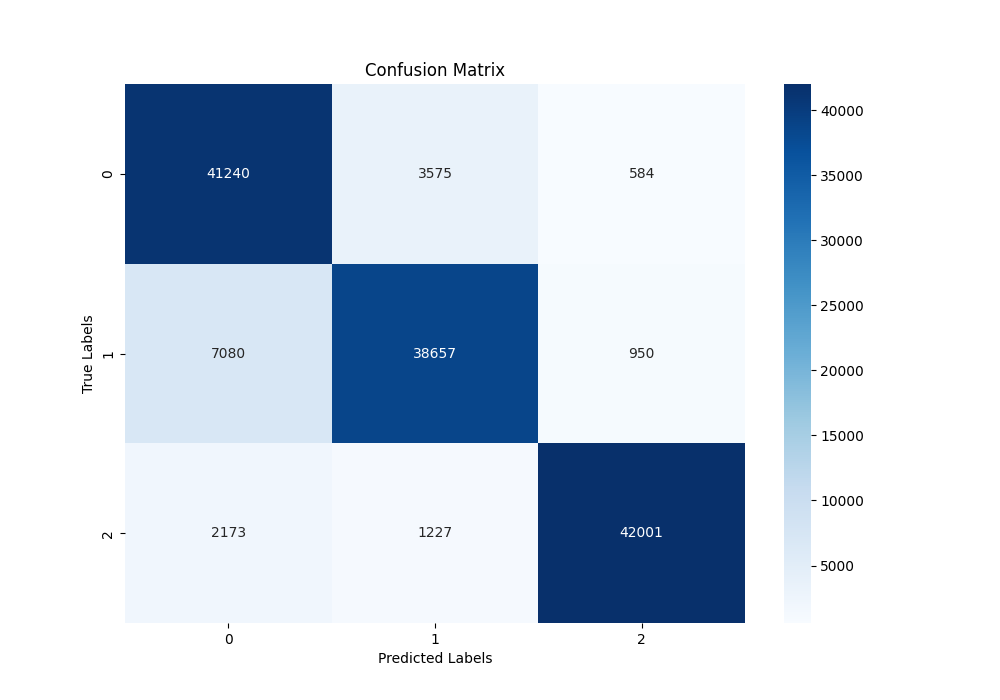
\includegraphics[width=0.9\linewidth]{CNN_Modelconfusion_matrix_cnn.png}
    \caption{Confusion Matrix for CNN Model}
    \label{fig:image1}
  \end{minipage}
  \hfill
  \begin{minipage}[b]{0.45\textwidth}
    \centering
    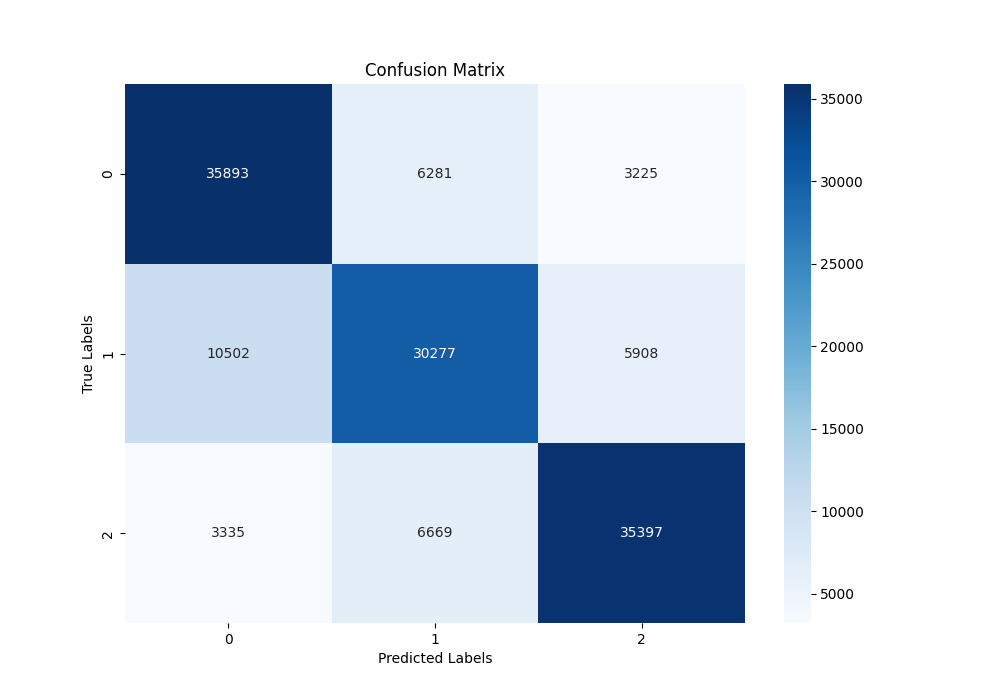
\includegraphics[width=0.9\linewidth]{MLP_Classifierconfusion_matrix_cnn.png}
    \caption{Confusion Matrix for MLP Model}
    \label{fig:image2}
  \end{minipage}
\end{figure}
\begin{figure}[H]
  \centering
  \begin{minipage}[b]{0.45\textwidth}
    \centering
    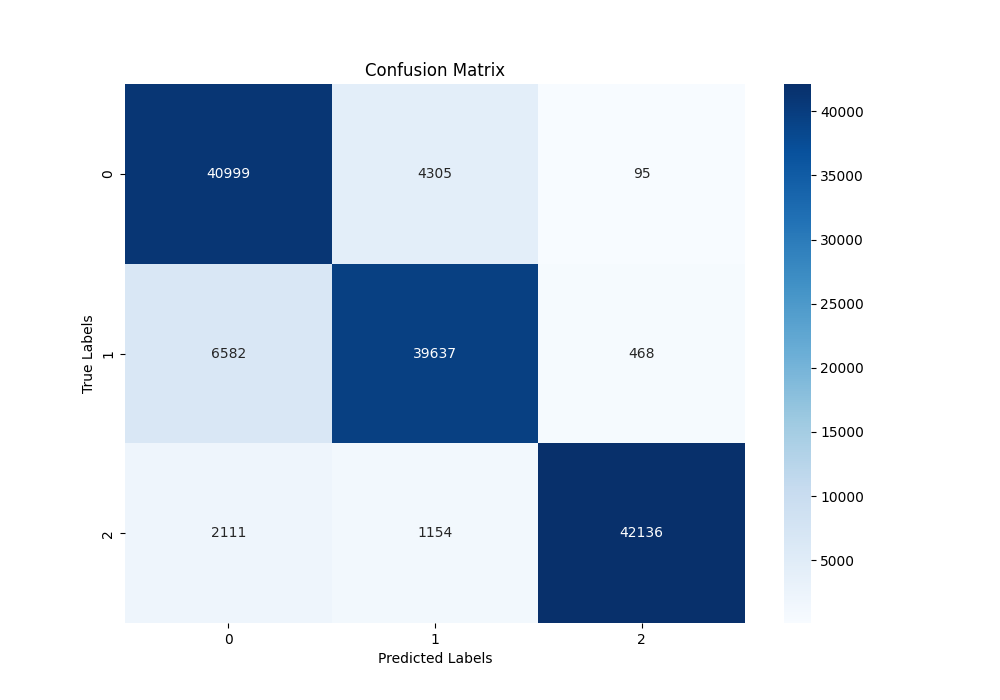
\includegraphics[width=0.9\linewidth]{LSTM_Text_Classifierconfusion_matrix_cnn.png}
    \caption{Confusion Matrix for BiLSTM Model}
    \label{fig:image1}
  \end{minipage}
  \hfill
  \begin{minipage}[b]{0.45\textwidth}
    \centering
    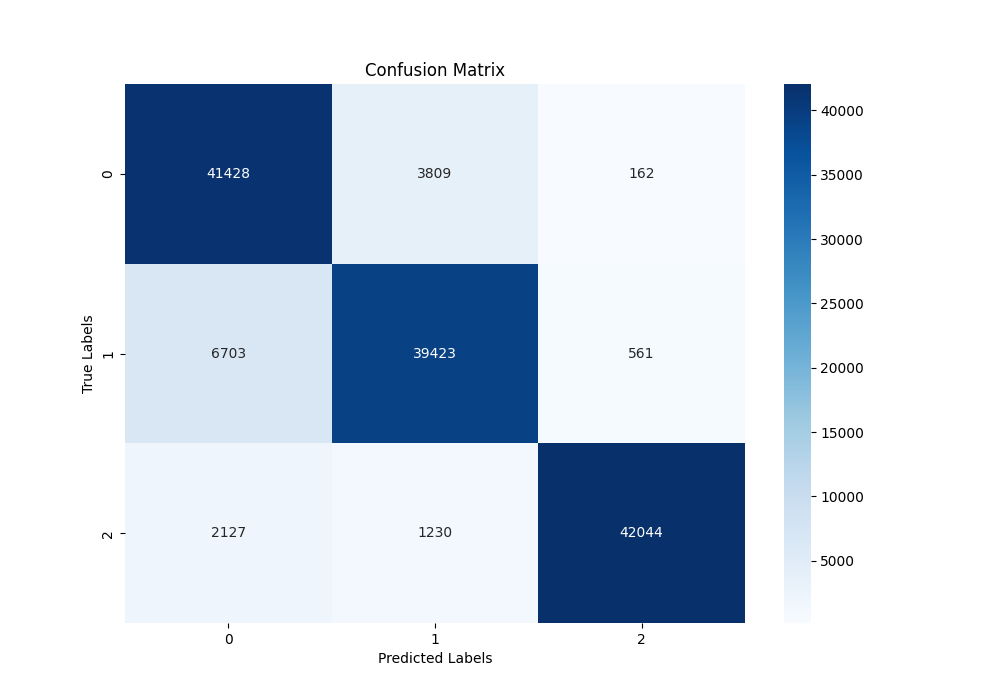
\includegraphics[width=0.9\linewidth]{LSTM_Multi_Head_Attentionconfusion_matrix_cnn.png}
    \caption{Confusion Matrix for BiLSTM-MHAM Model}
    \label{fig:image2}
  \end{minipage}
\end{figure}
\begin{figure}[H]
  \centering
  \begin{minipage}[b]{0.45\textwidth}
    \centering
    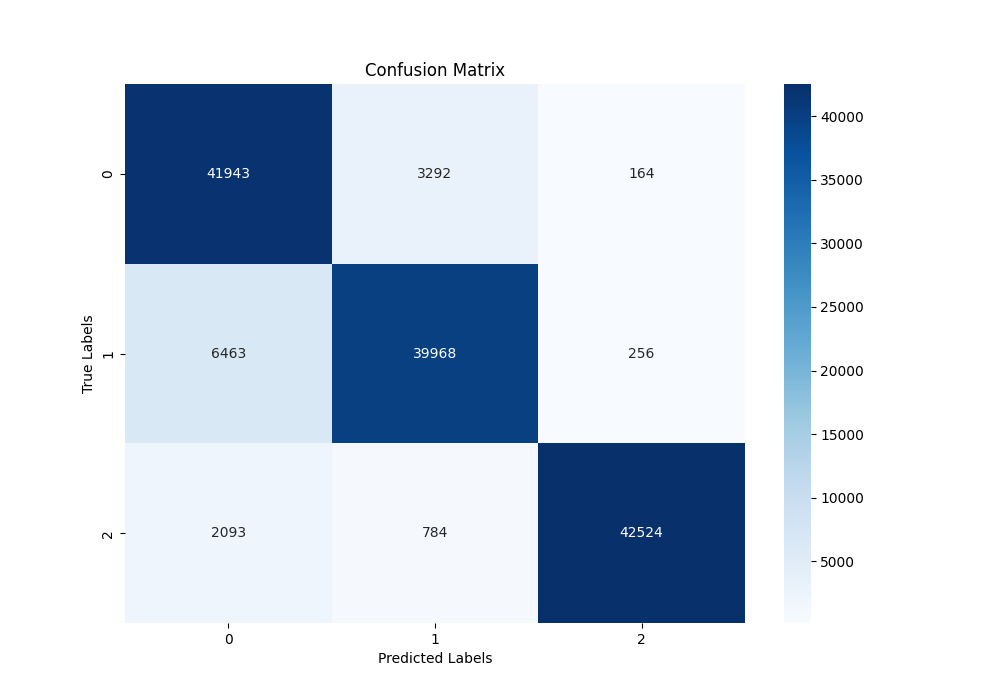
\includegraphics[width=0.9\linewidth]{RCNN_Text_Classifierconfusion_matrix_cnn.png}
    \caption{Confusion Matrix for RCNN Model}
    \label{fig:image1}
  \end{minipage}
  \hfill
  \begin{minipage}[b]{0.45\textwidth}
    \centering
    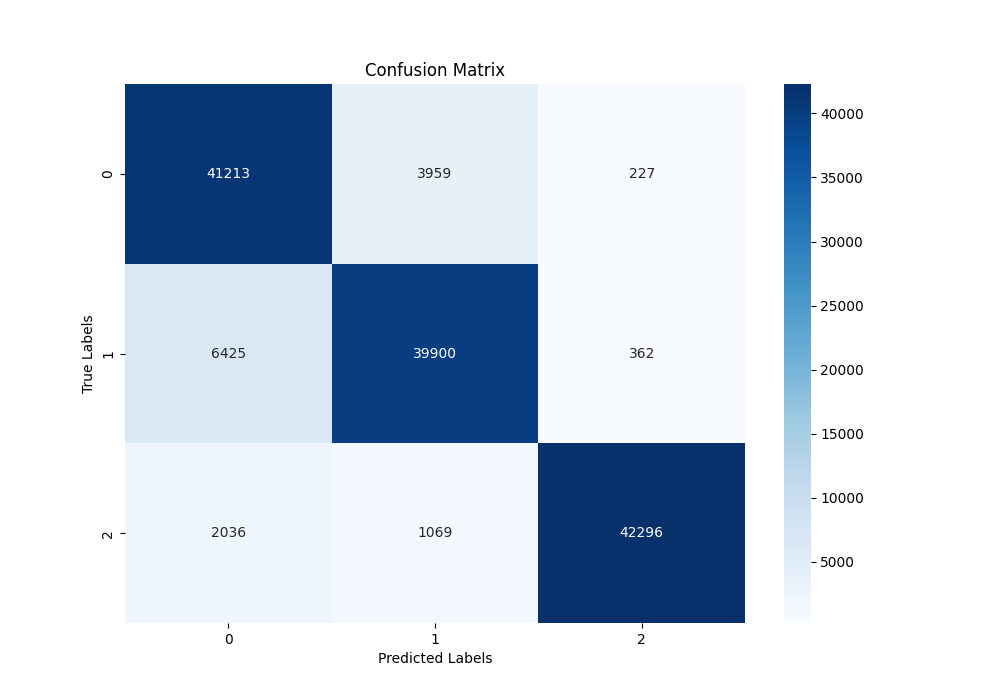
\includegraphics[width=0.9\linewidth]{BiGRU_Attention_Residualconfusion_matrix_cnn.png}
    \caption{Confusion Matrix for BiGRU-AR Model}
    \label{fig:image2}
  \end{minipage}
\end{figure}

Training vs Validation loss for different models used in the study:
\begin{figure}[H]
  \centering
  \begin{minipage}[b]{0.45\textwidth}
    \centering
    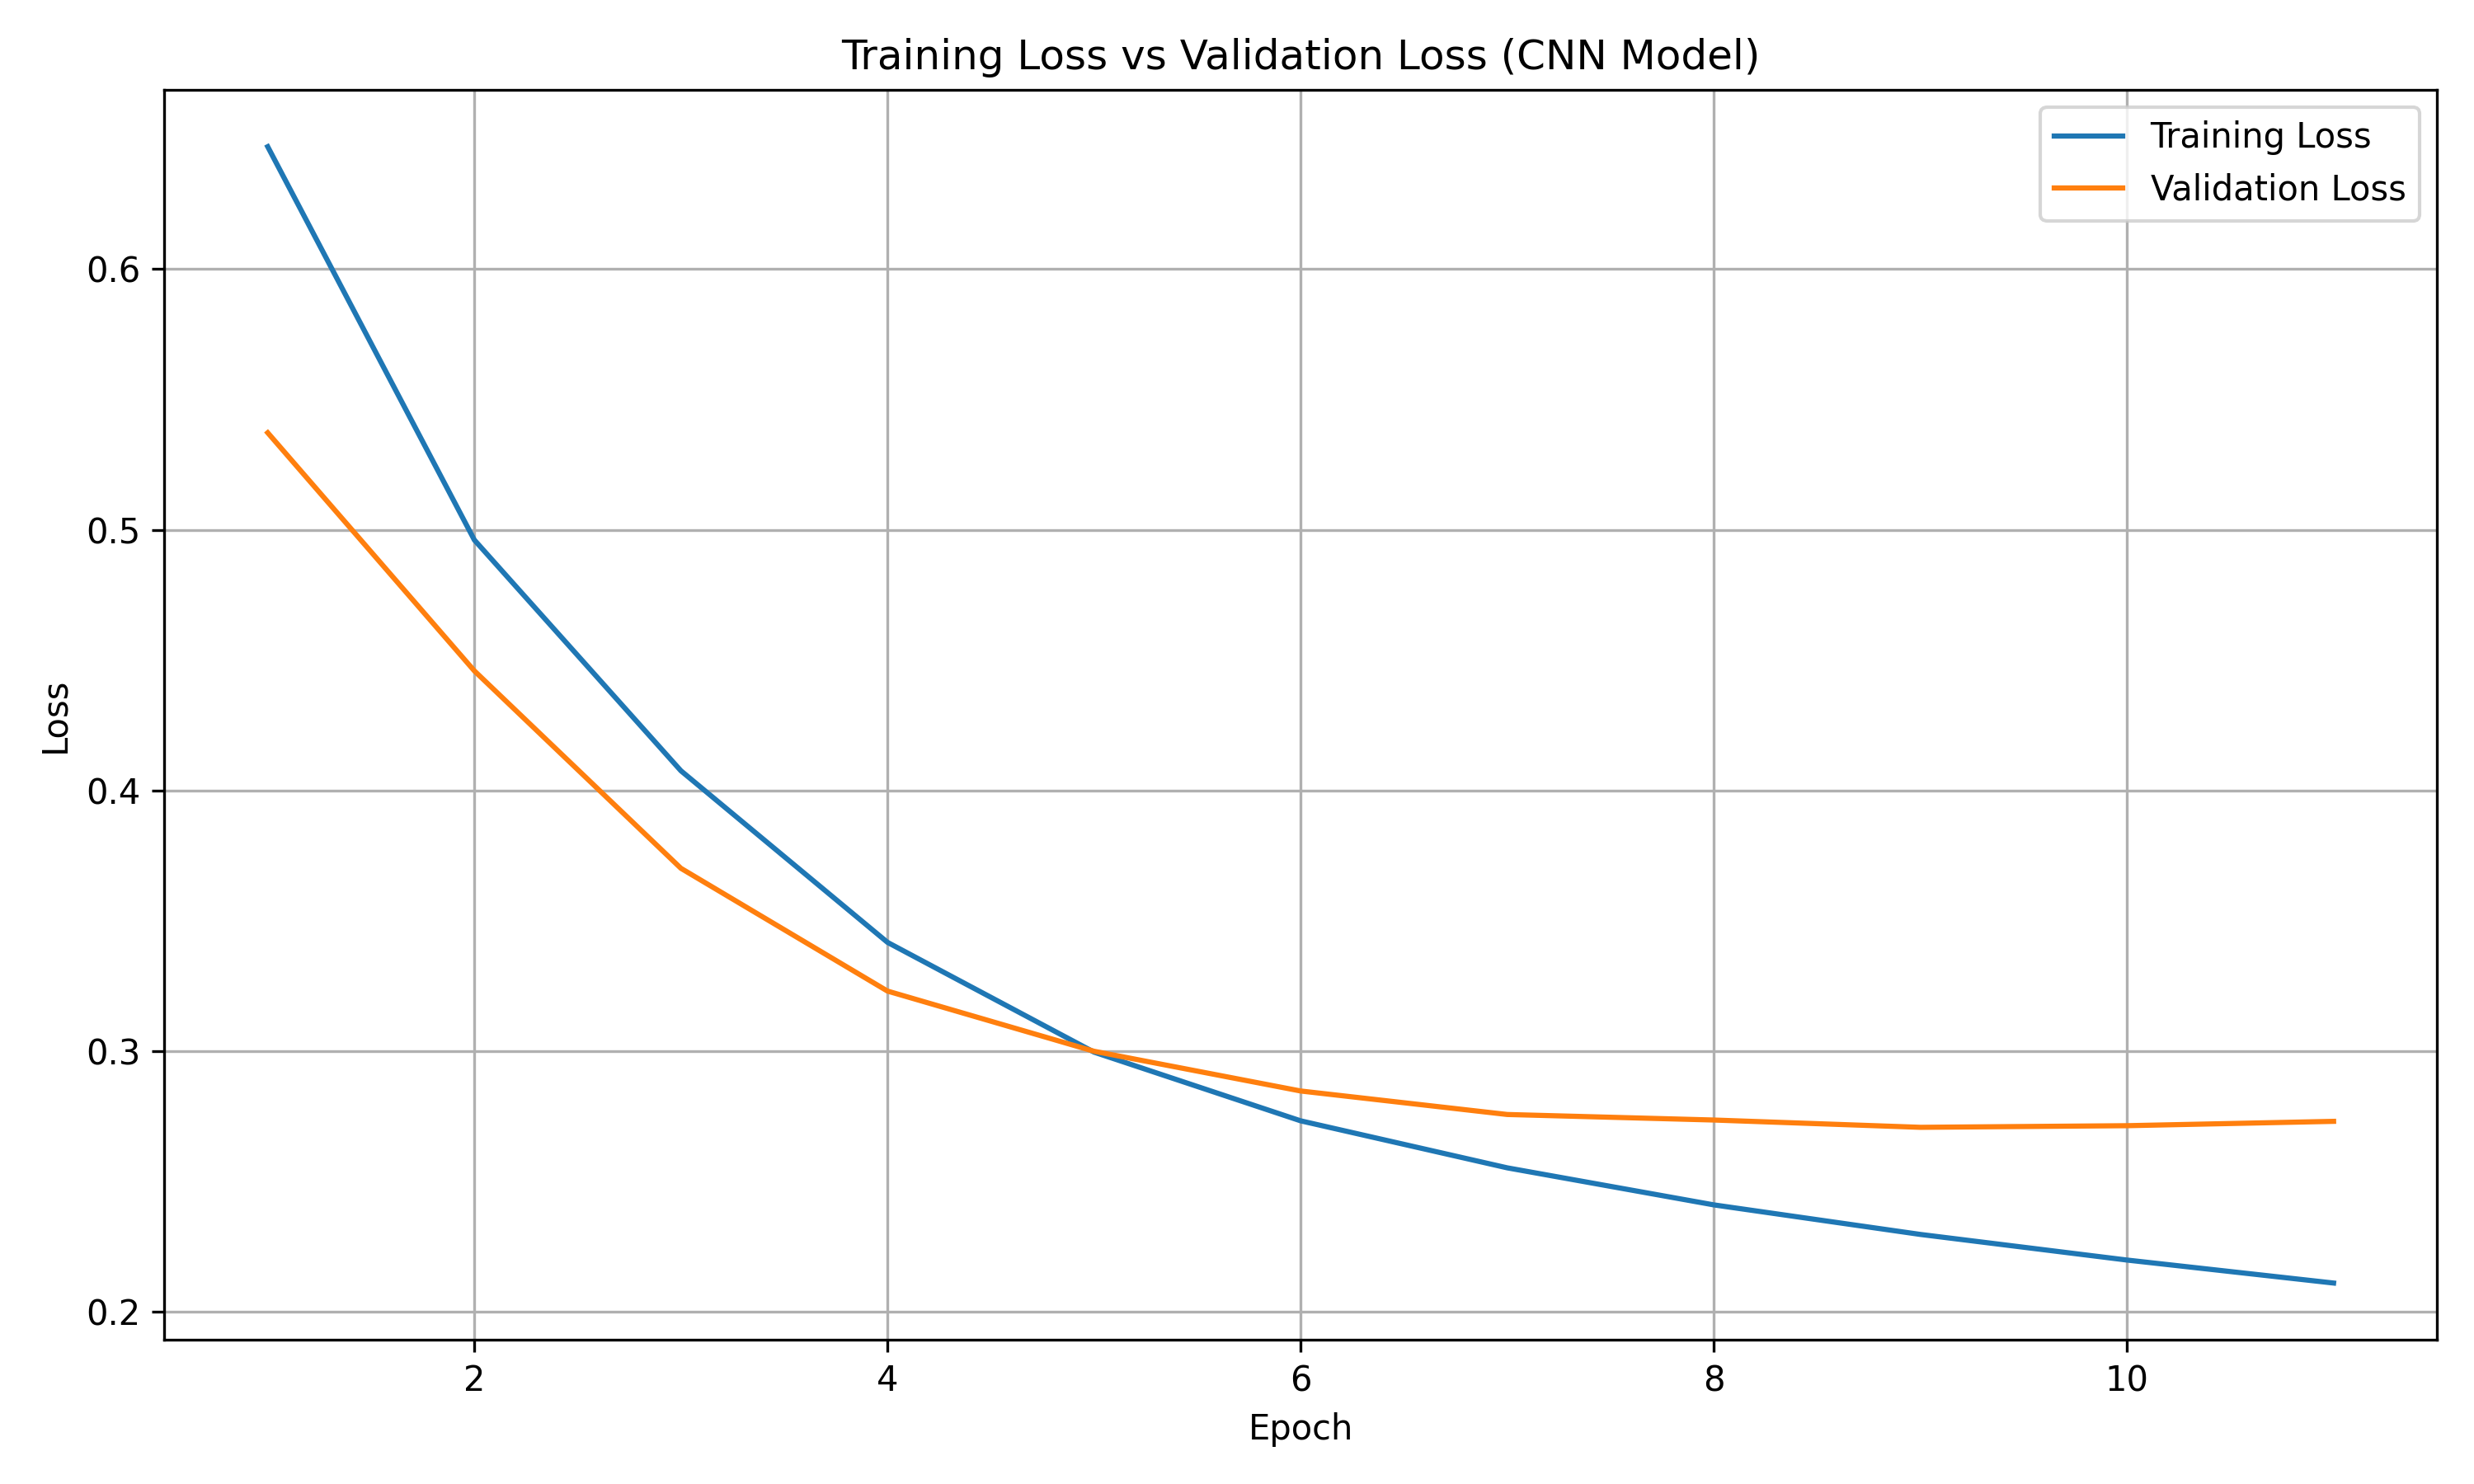
\includegraphics[width=0.9\linewidth]{cnn_loss_curve.png}
    \caption{Training vs Validation Loss - CNN Model}
    \label{fig:image1}
  \end{minipage}
  \hfill
  \begin{minipage}[b]{0.45\textwidth}
    \centering
    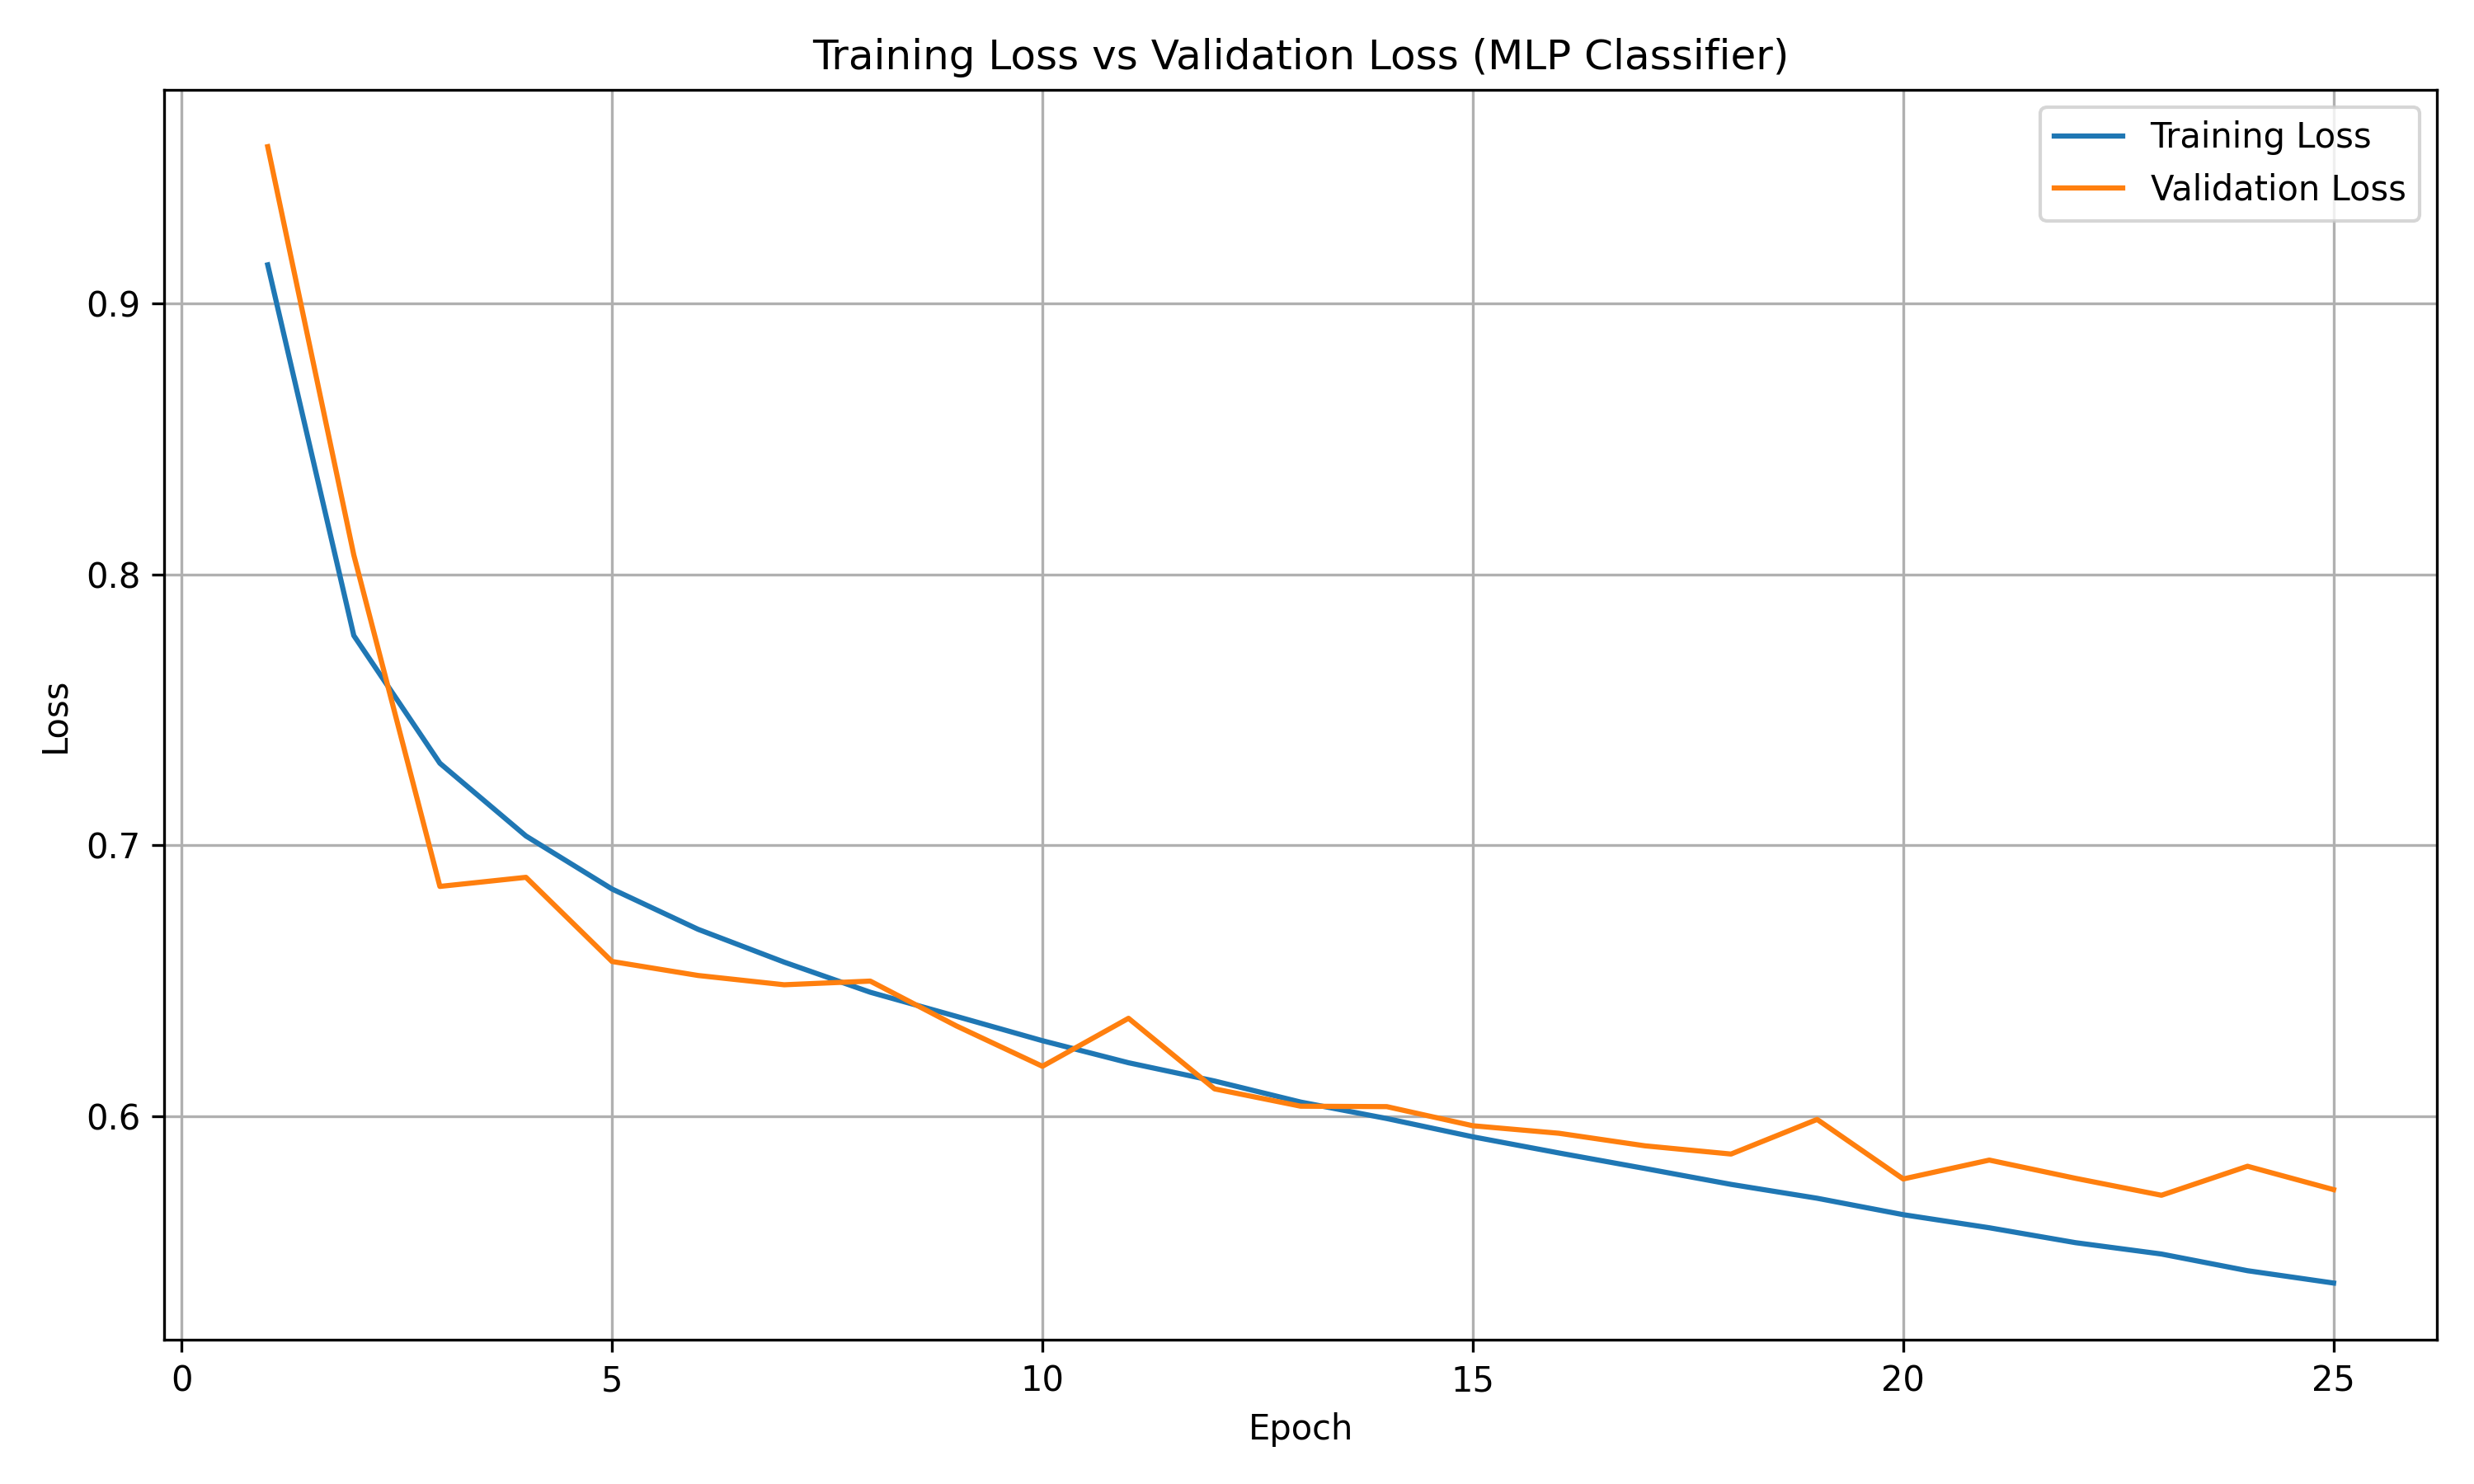
\includegraphics[width=0.9\linewidth]{mlp_loss_curve.png}
    \caption{Training vs Validation Loss - MLP Model}
    \label{fig:image2}
  \end{minipage}
\end{figure}
\begin{figure}[H]
  \centering
  \begin{minipage}[b]{0.45\textwidth}
    \centering
    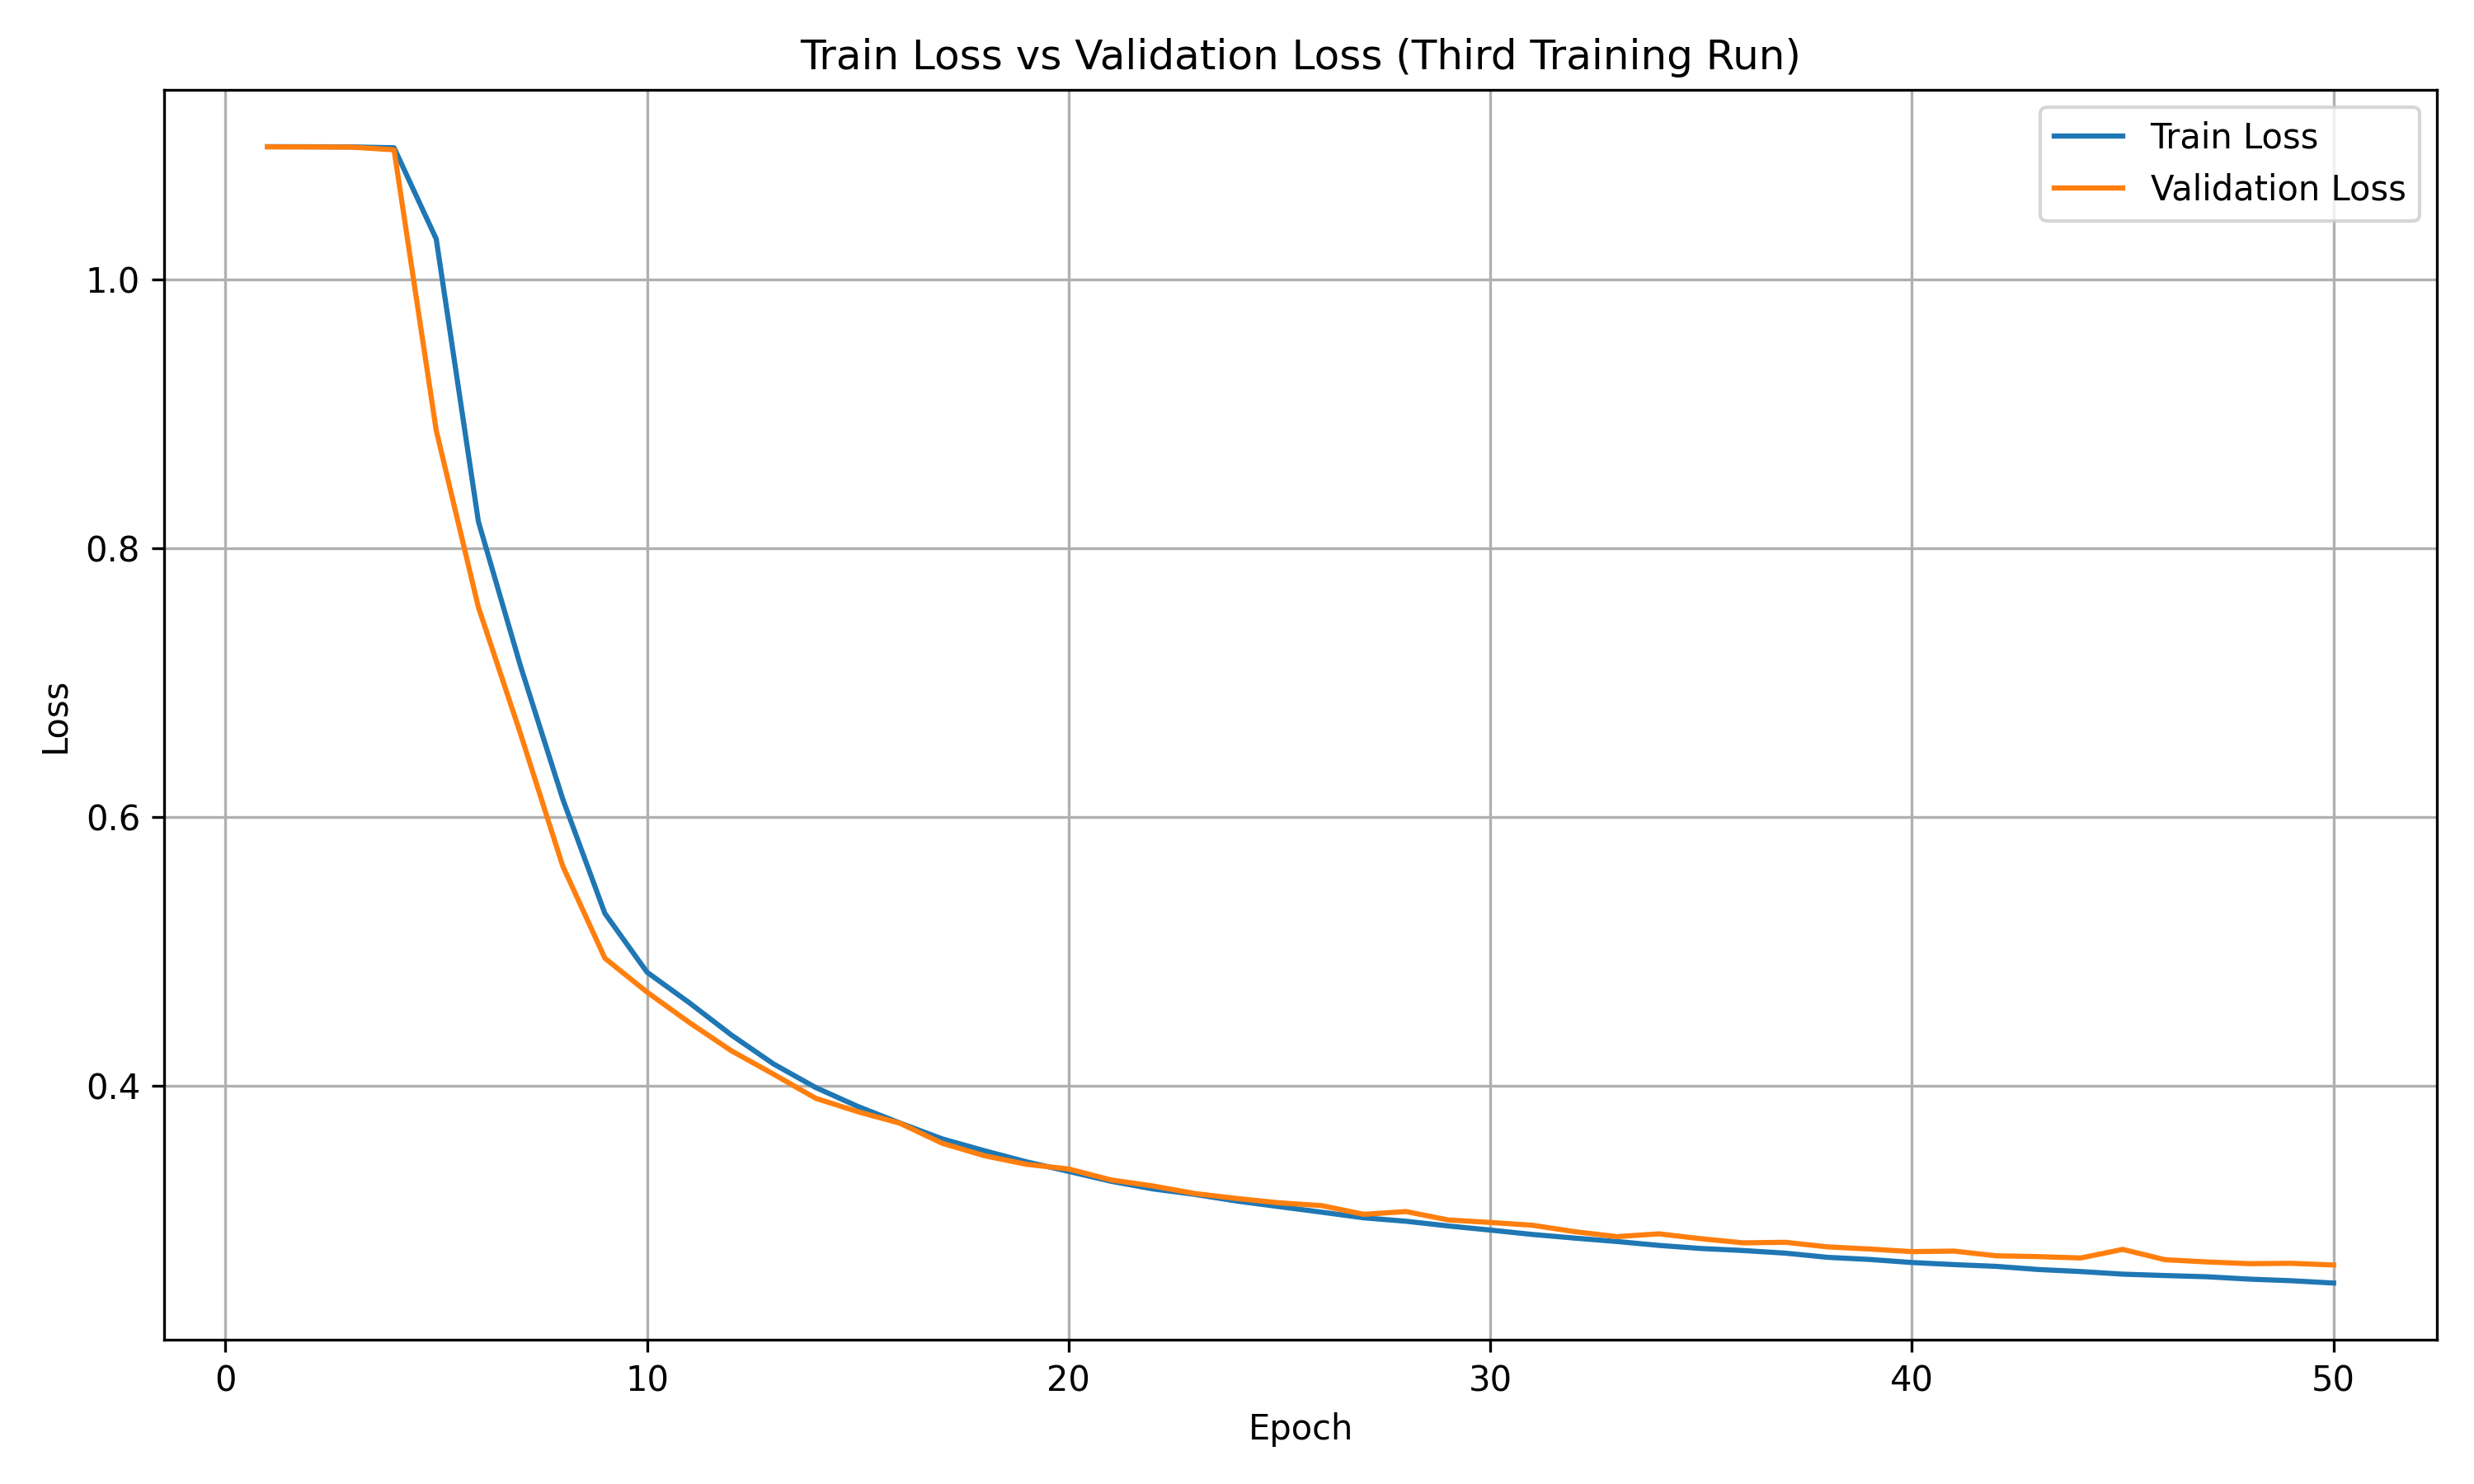
\includegraphics[width=0.9\linewidth]{lstm_tc_loss_curve.png}
    \caption{Training vs Validation Loss - BiLSTM Model}
    \label{fig:image1}
  \end{minipage}
  \hfill
  \begin{minipage}[b]{0.45\textwidth}
    \centering
    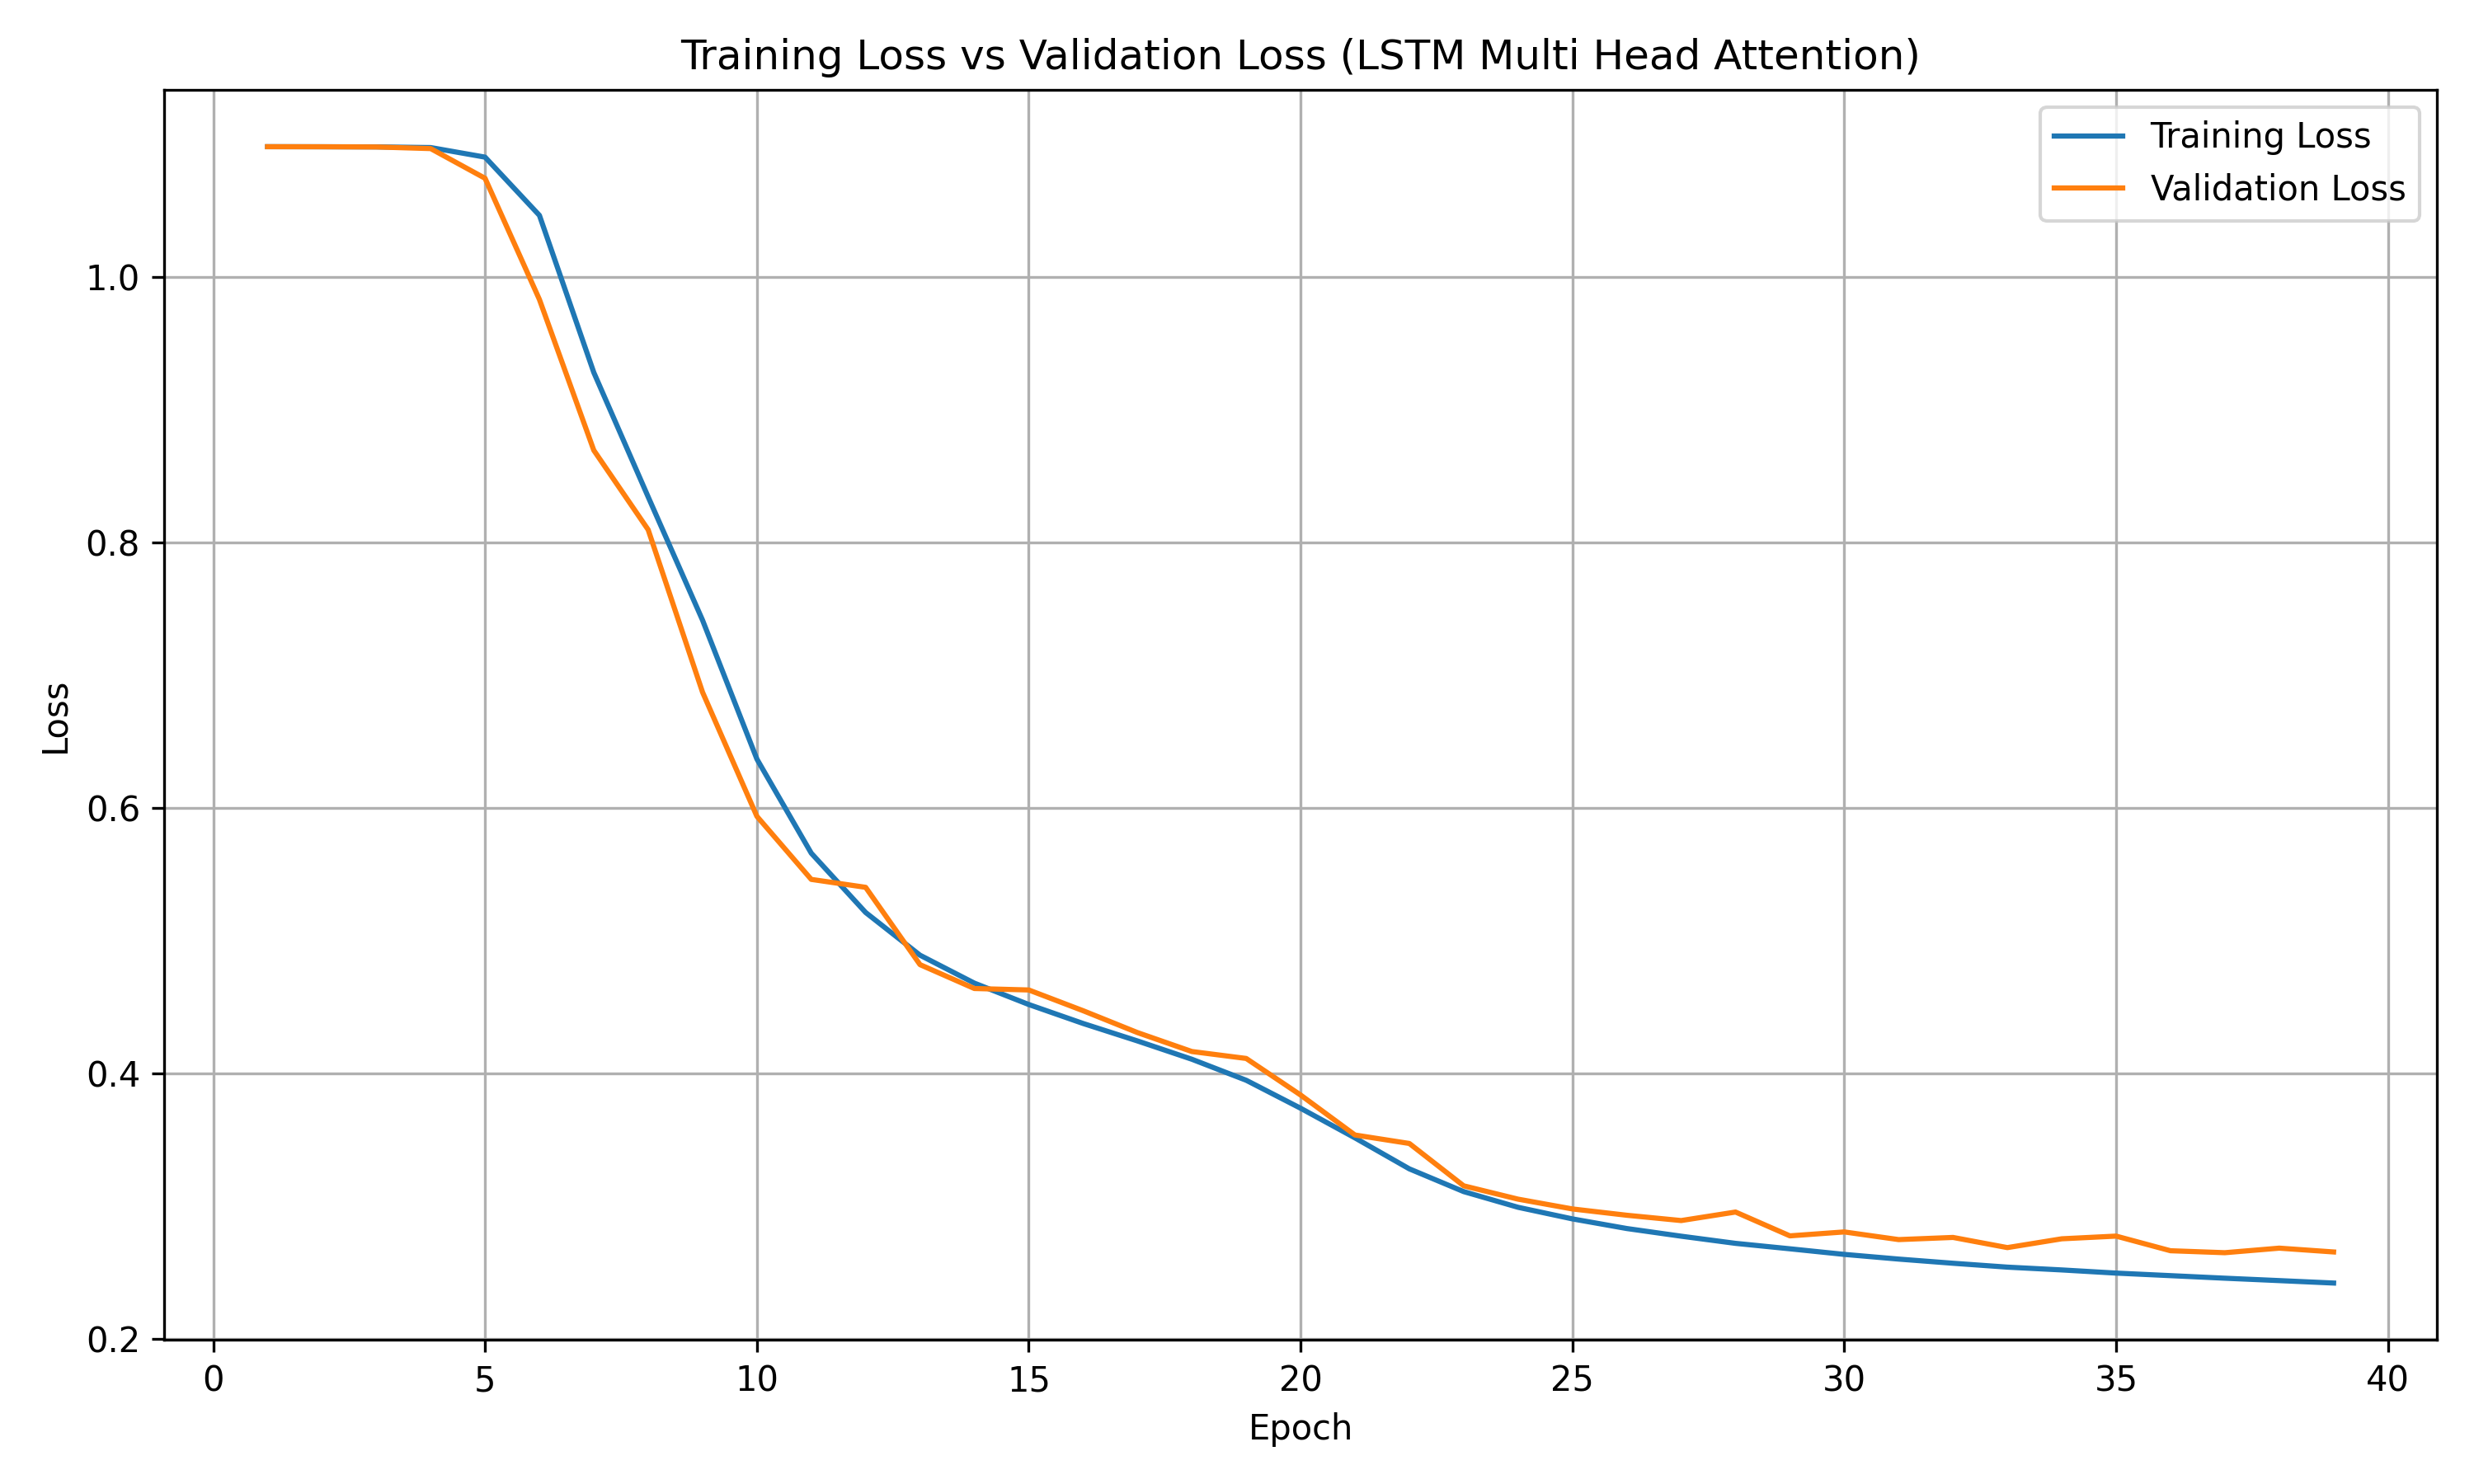
\includegraphics[width=0.9\linewidth]{lstm_ma_loss_curve.png}
    \caption{Training vs Validation Loss - BiLSTM-MHAM Model}
    \label{fig:image2}
  \end{minipage}
\end{figure}
\begin{figure}[H]
  \centering
  \begin{minipage}[b]{0.45\textwidth}
    \centering
    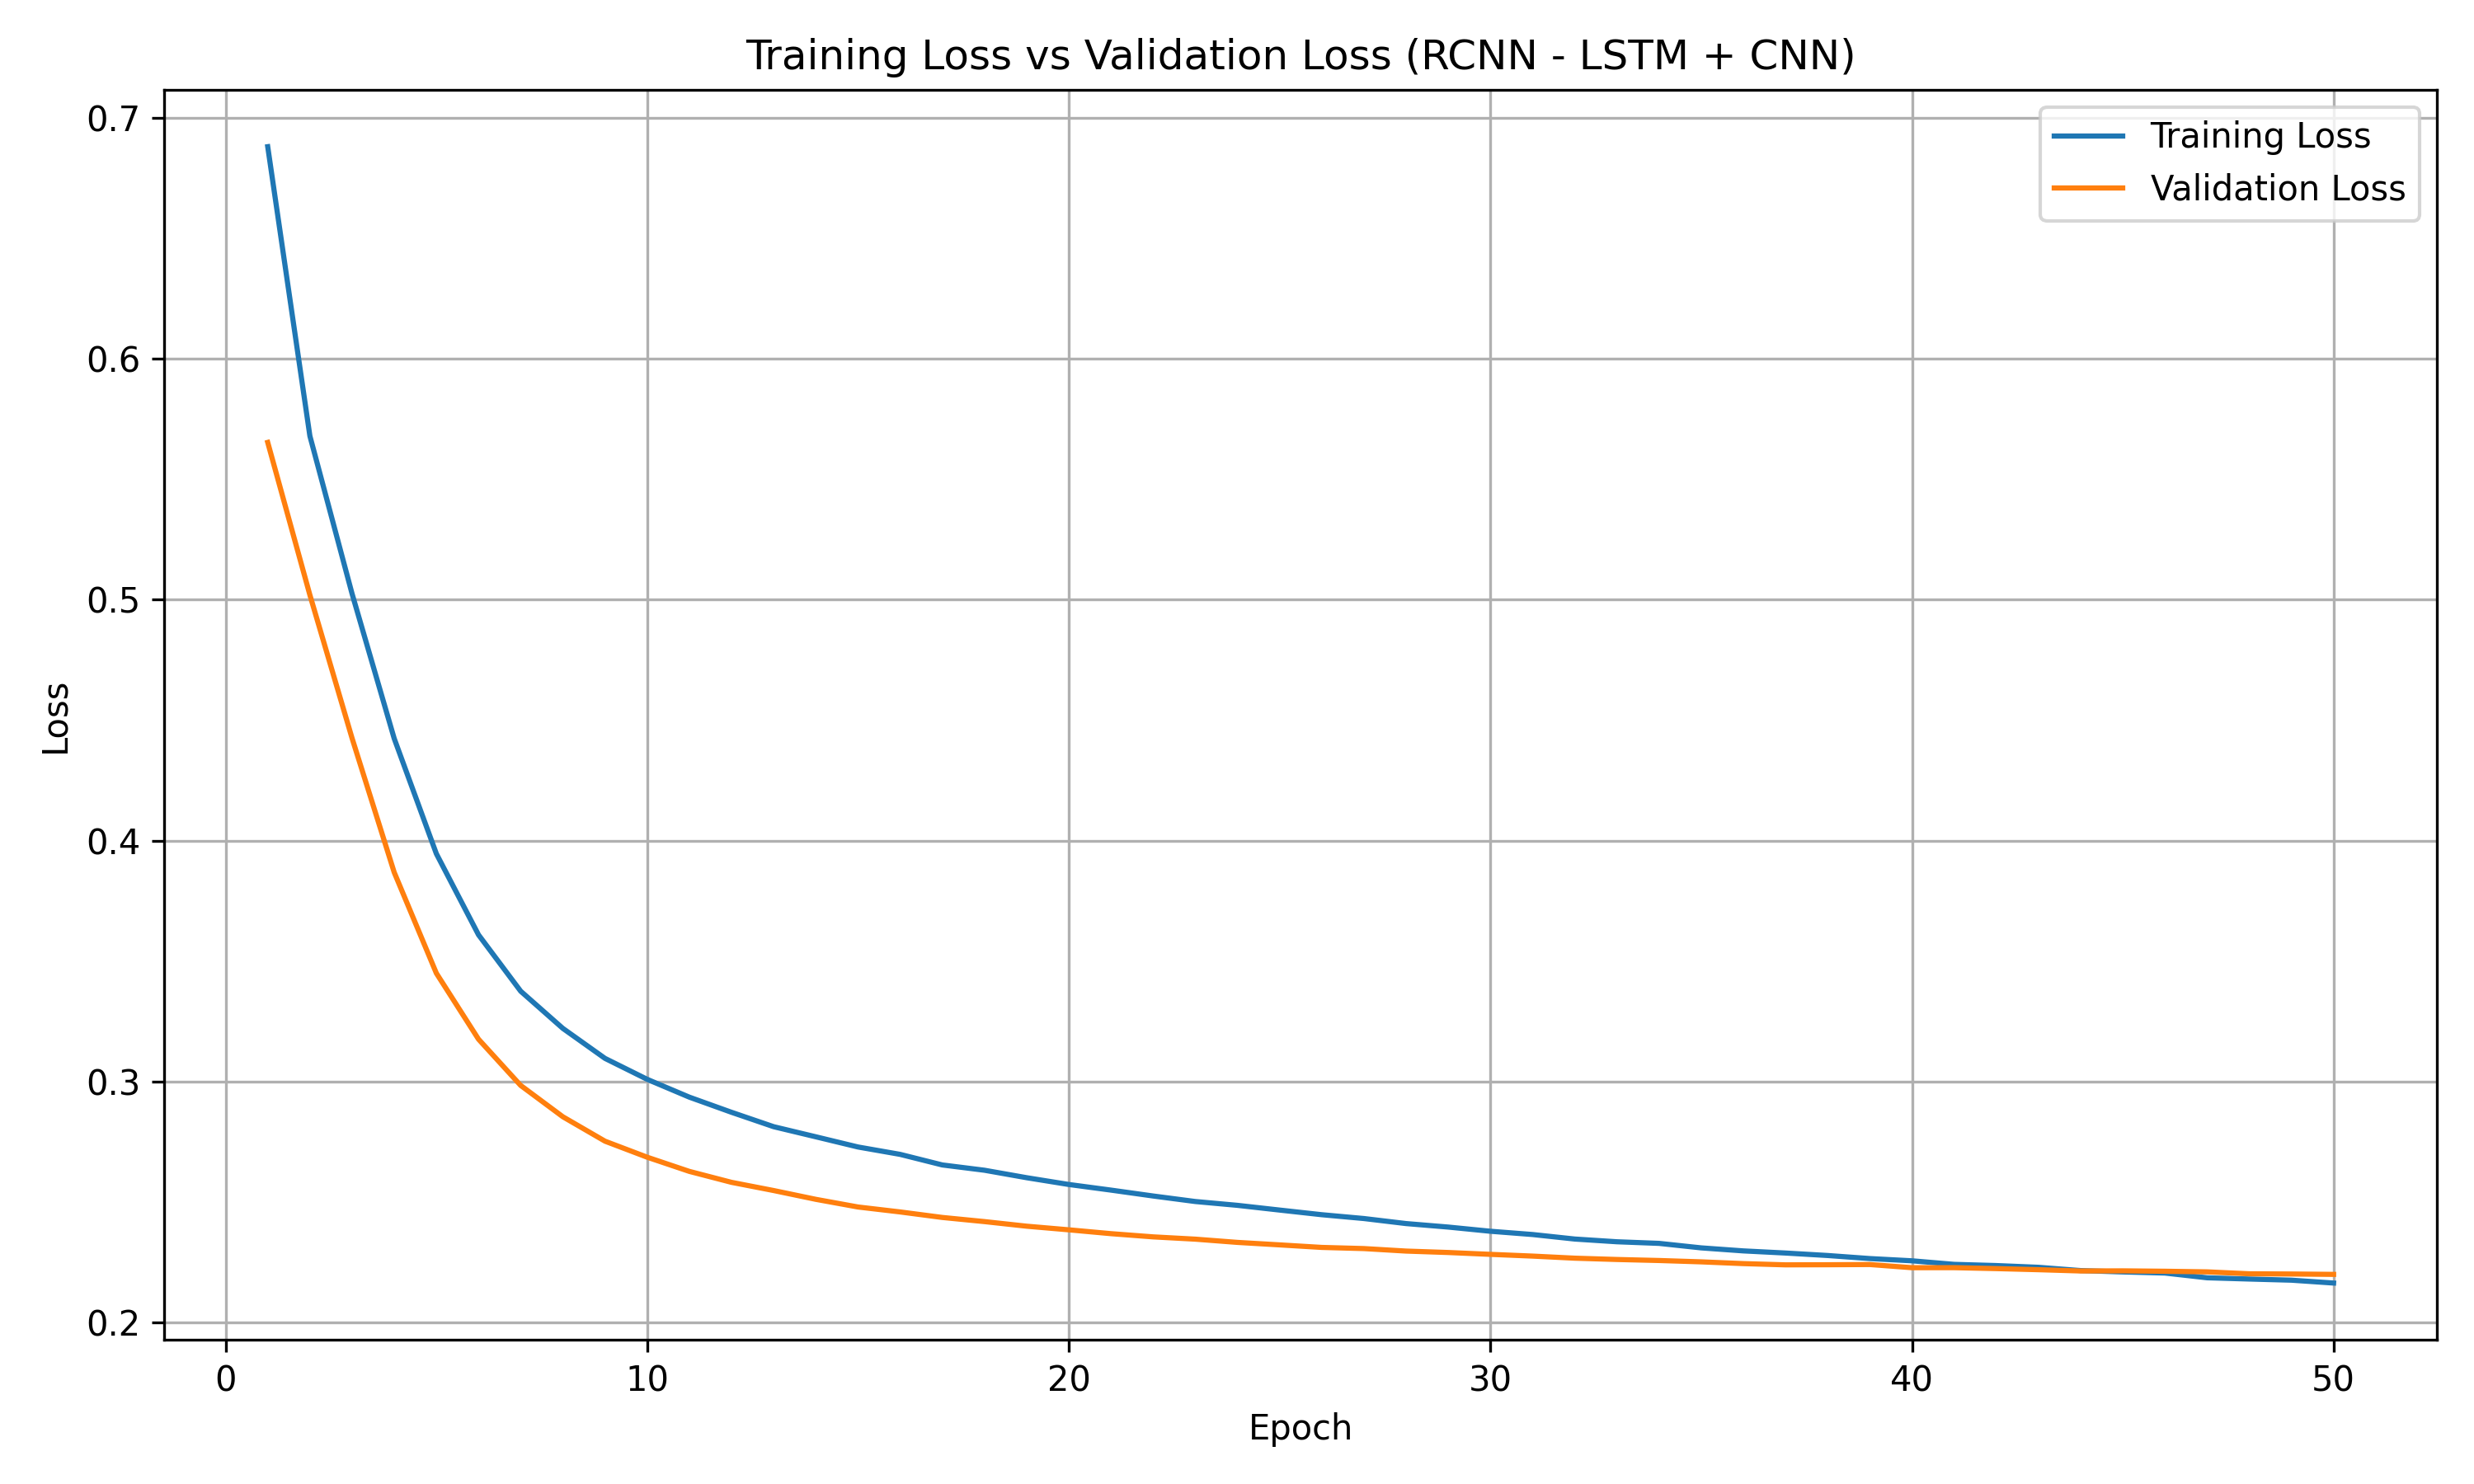
\includegraphics[width=0.9\linewidth]{rcnn_loss_curve.png}
    \caption{Training vs Validation Loss - RCNN Model}
    \label{fig:image1}
  \end{minipage}
  \hfill
  \begin{minipage}[b]{0.45\textwidth}
    \centering
    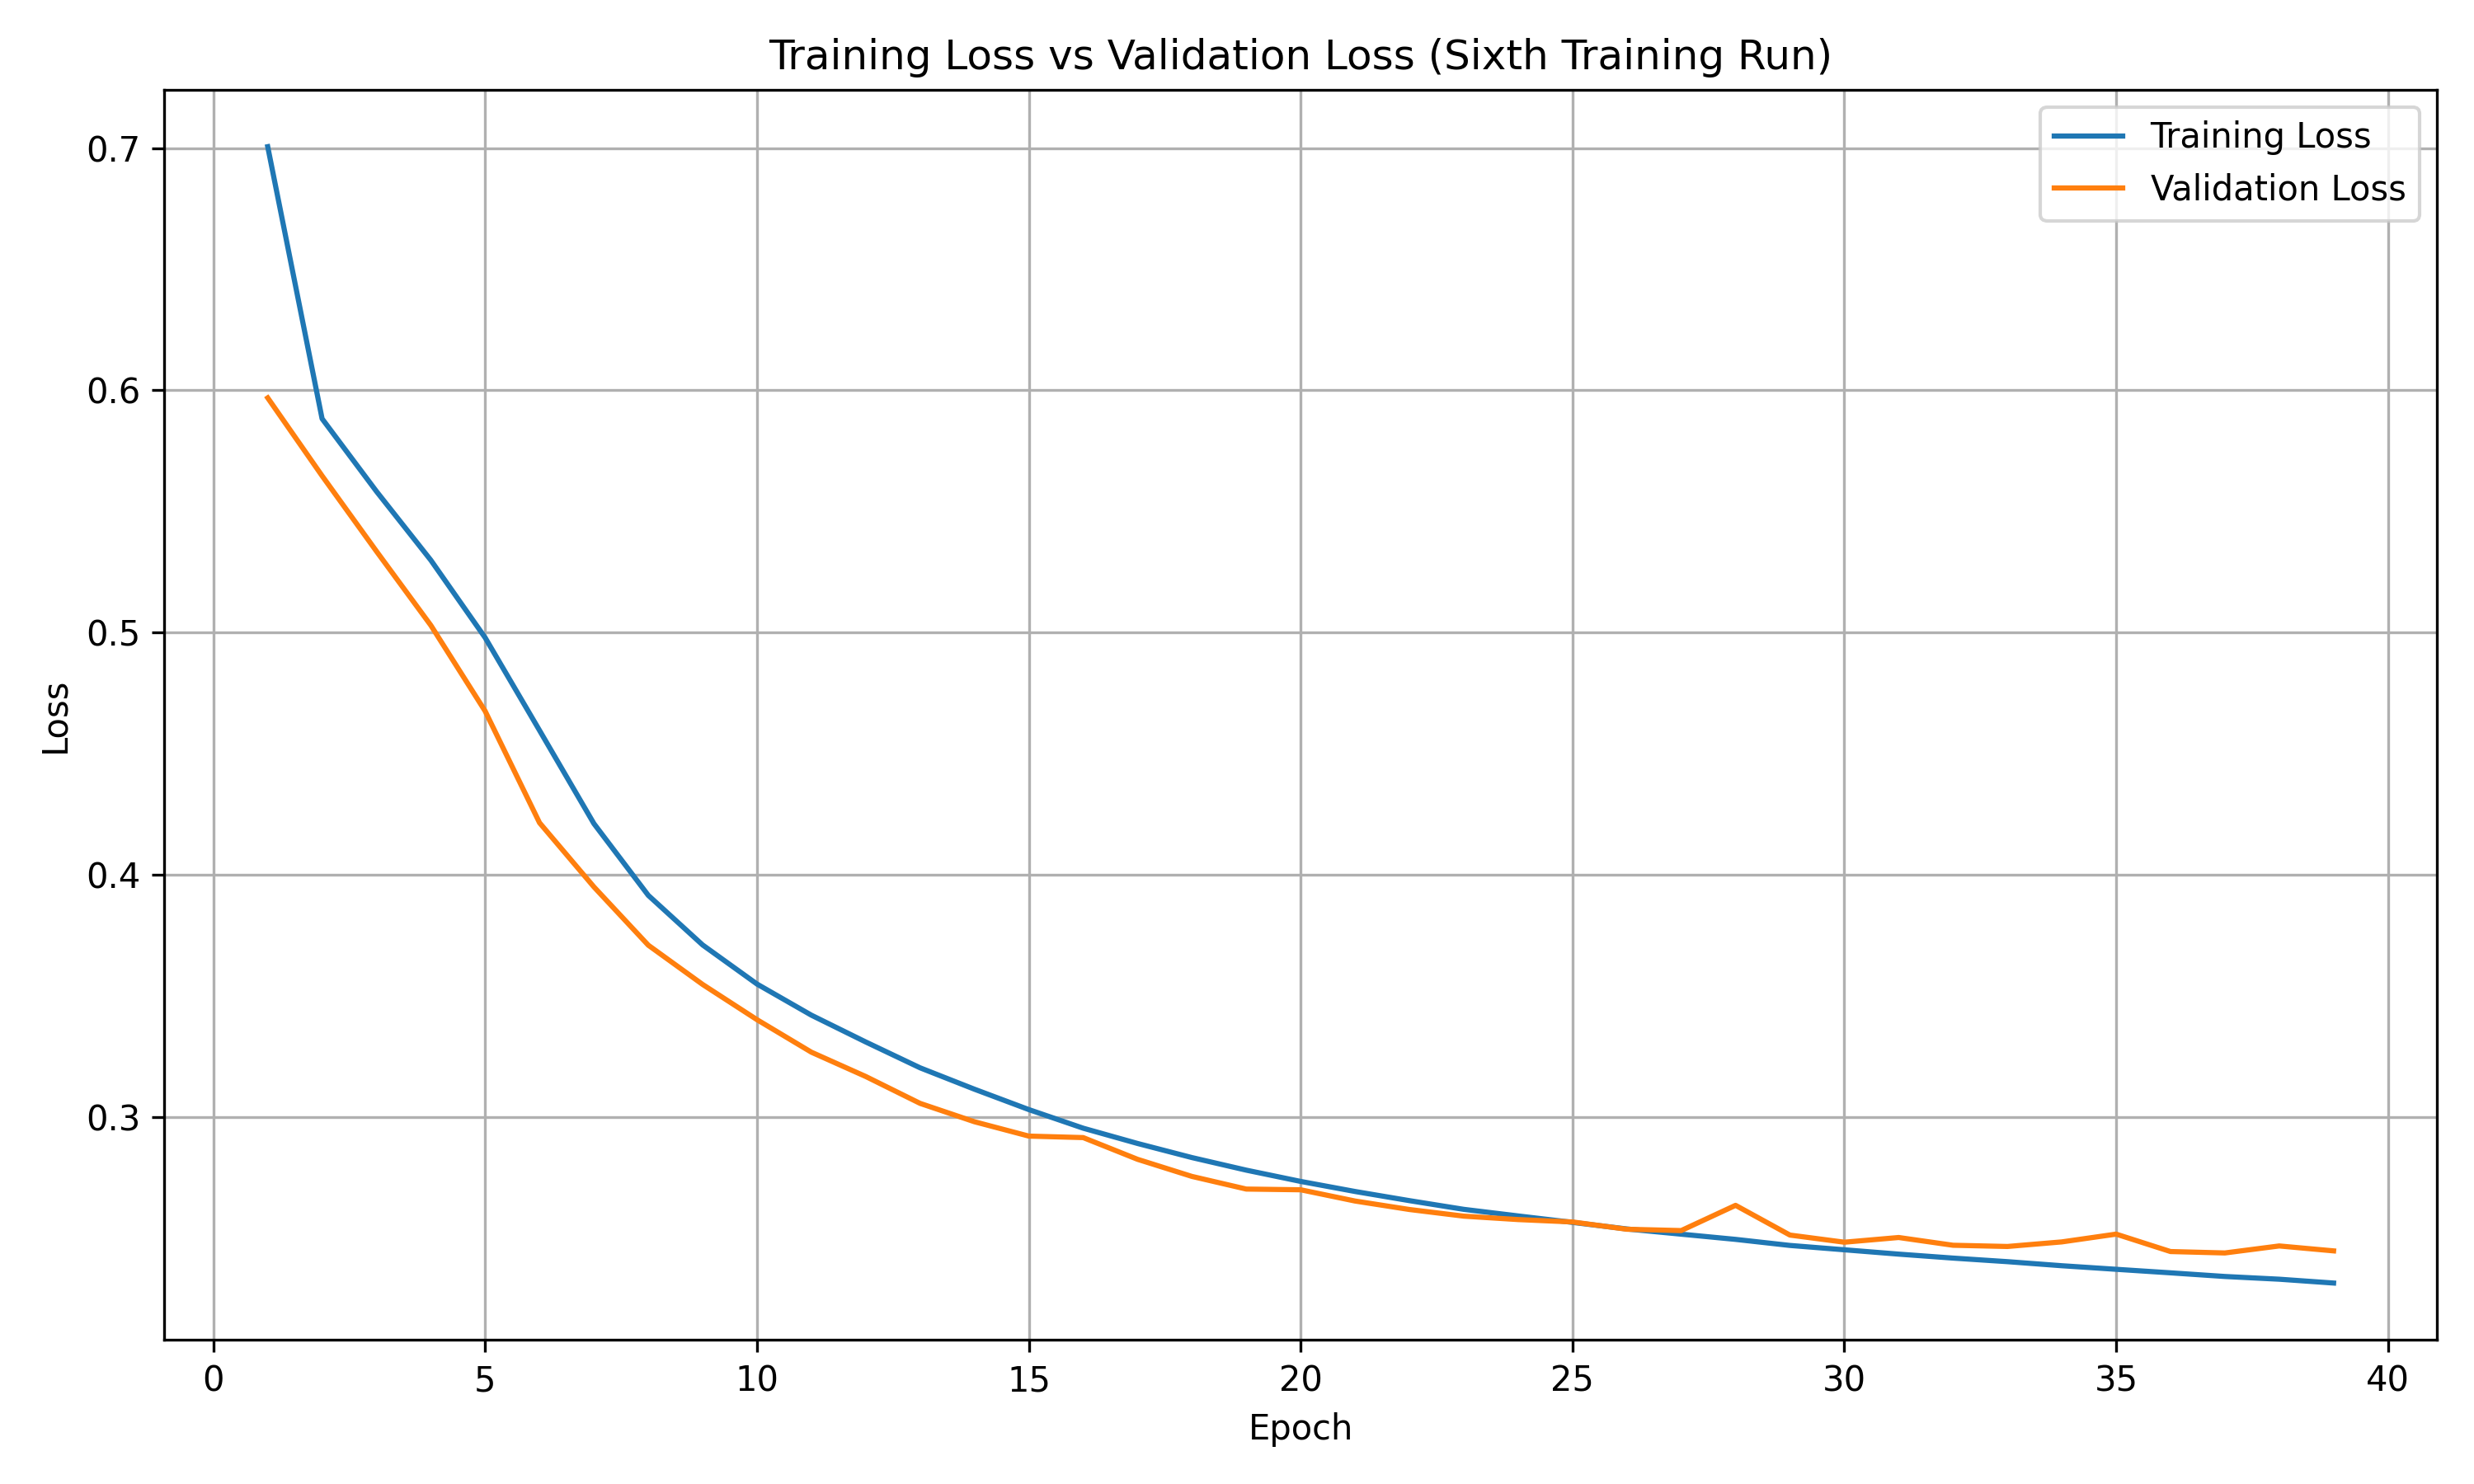
\includegraphics[width=0.9\linewidth]{bigru_loss_curve.png}
    \caption{Training vs Validation Loss - BiGRU Attention Residual Model}
    \label{fig:image2}
  \end{minipage}
\end{figure}

Future research in tweet-based sentiment analysis can branch into several impactful directions to enhance accuracy, robustness, and applicability. One promising area is domain-adaptive pre-training, where models are pre-trained specifically on large volumes of Twitter or social media text. Since general-purpose language models often struggle with informal and abbreviated language, this approach can help the model better understand the unique linguistic features of tweets, such as slang, emojis, and non-standard grammar.

Another key area is multilingual and code-mixed sentiment analysis. Twitter is used globally, and many users tweet in languages other than English or mix languages within a single tweet (e.g., Hinglish). Building models that can handle such linguistic diversity would significantly broaden the utility of sentiment analysis tools. This can be achieved through multilingual embeddings or transformer-based models trained on diverse linguistic datasets.

There is also great potential in temporal sentiment tracking, where models can analyse how public sentiment evolves over time, particularly around events like political debates, product releases, or crises. Incorporating time-aware features or using sequential models conditioned on timestamps can provide valuable insights for trend analysis and forecasting.

Finally, incorporating multimodal information, such as images, hashtags, or user metadata that can lead to richer sentiment analysis. Tweets often rely on visual context or user-specific information to convey sentiment fully. Developing models that integrate both text and non-textual data (e.g., using image-text fusion techniques) can provide a more holistic understanding of sentiment.

\section{References}

\small
[1] Thumbs up? Sentiment Classification using Machine Learning Techniques(https://aclanthology.org/W02-1011) (Pang et al., EMNLP 2002)

[2] Recursive Deep Models for Semantic Compositionality Over a Sentiment Treebank(https://aclanthology.org/D13-1170) (Socher et al., EMNLP 2013).

[3] Kim, Y. (2014) Convolutional Neural Networks for Sentence Classification. Proceedings of the 2014
Conference on Empirical Methods in Natural Language Processing (EMNLP), Doha, 1746-1751. arXiv:
1408.5882 https://doi.org/10.3115/v1/D14-1181.

[4] Ashish Vaswani, Noam Shazeer, Niki Parmar, Jakob Uszkoreit, Llion Jones, Aidan N. Gomez, Łukasz Kaiser, and Illia Polosukhin. 2017. Attention is all you need. In Proceedings of the 31st International Conference on Neural Information Processing Systems (NIPS’17). Curran Associates Inc., Red Hook, NY, USA, 6000–6010.

[5] Hochreiter, S. and Schmidhuber, J. (1997) Long Short-Term Memory. Neural Computation, 9, 1735-1780. https://doi.org/10.1162/neco.1997.9.8.1735

[6] M. Schuster and K. K. Paliwal, "Bidirectional recurrent neural networks," in IEEE Transactions on Signal Processing, vol. 45, no. 11, pp. 2673-2681, Nov. 1997, doi: 10.1109/78.650093. keywords: Recurrent neural networks;Artificial neural networks;Training data;Databases;Probability;Shape;Parameter estimation;Speechrecognition;Control systems;Telecommunication control,

[7] Li, Xu, Tianxuan Hao, Fan Li, Lizhen Zhao, and Zehua Wang. 2023. "Faster R-CNN-LSTM Construction Site Unsafe Behavior Recognition Model" Applied Sciences 13, no. 19: 10700. https://doi.org/10.3390/app131910700

[8] Dzmitry Bahdanau, KyunghyunCho, and Yoshua Bengio. 2015. Neural machine translation by jointly
learning to align and translate. In ICLR.

[9] Kumar, A., Sachdeva, N. A Bi-GRU with attention and CapsNet hybrid model for cyberbullying detection on social media. World Wide Web 25, 1537–1550 (2022). https://doi.org/10.1007/s11280-021-00920-4

[10] Pustokhin, D. A., Pustokhina, I. V., Dinh, P. N., Phan, S. V., Nguyen, G. N., Joshi, G. P., and K., S. (2020). An effective deep residual network based class attention layer with bidirectional LSTM for diagnosis and classification of COVID-19. Journal of Applied Statistics, 50(3), 477–494. https://doi.org/10.1080/02664763.2020.1849057



\end{document}